\documentclass[a4paper,12pt]{article}
\usepackage[T1]{fontenc}
\usepackage{fullpage,graphicx,psfrag,amsmath,amsfonts}
\usepackage[small,bf]{caption}
\usepackage[utf8]{inputenc}
\usepackage[english]{babel}
\usepackage{lipsum}
\usepackage{url}
\usepackage{bm}
\usepackage{float}
\usepackage{kpfonts}
\usepackage{mathpazo}
\usepackage{enumitem}
\setitemize{noitemsep,topsep=0pt,parsep=0pt,partopsep=0pt}

\begin{document}
\author{Filippo Grotto VR460638}

\title{Physical Human Robot Interaction}

\maketitle
\tableofcontents

\section{Introduction}
In bilateral telemanipulation the aim is to allow to interact with a remote environment by using a joystic. The user manipulates the environment and perceives the reaction force through the haptic device (force feedback). The role of the control is to guarantee and/or enhance the coupling characteristics between the user at the master side and the environment at the slave side. Several components plays a role in a bilateral telemanipulation architecture: human operator, haptic device, master controller, communication channel (using a proper protocol), slave controller, slave robot and environment. A crucial part is the communication channel that has to be robust to delays and packet losses. 

\bigskip
\noindent The hybrid two-port representation that we are going to use are the following
\[
    \begin{bmatrix}
        f_m \\ \dot{x}_m
    \end{bmatrix} = \begin{bmatrix}
        H_{11}(s) & H_{12}(s) \\ H_{21}(s) & H_{22}(s)
    \end{bmatrix} = \begin{bmatrix}
        \dot{x_s} \\ -f_s
    \end{bmatrix} \qquad \text{Hannaford hybrid matrix}
\]
\[
    \begin{bmatrix}
        f_m \\ -\dot{x}_s
    \end{bmatrix} = \begin{bmatrix}
        \bar{H_{11}}(s) & \bar{H_{12}}(s) \\ \bar{H_{21}}(s) &\bar{ H_{22}}(s)
    \end{bmatrix} = \begin{bmatrix}
        \dot{x}_m \\ f_s
    \end{bmatrix} \qquad \text{Lawrence hybrid matrix}
\]
where 

\begin{itemize}
    \item $\bar{H_{11}}(s)$ is the uncontrained movement impedance the equivalent inertia and damping that the operator feels moving the master robot if the slave is in free motion. It should be as low as possible. 
    \item $\bar{H_{21}}(s)$ position tracking during unconstrained motion: ability of the slave robot to follow the position of the master robot. It should tend to unity, if no position scaling is desired, with infinite bandwidth. 
    \item $\bar{H_{12}}(s)$ tracking of forces in contact tasks when the operator keeps the master steady against the forces that the slave encounters. It should tend to unity, if no force scaling is desired, with infinite bandwidth.
    \item $\bar{H_{22}}(s)$ contact admittance: position tracking during contact tasks.
\end{itemize}

\bigskip
The key concepts of an architecture are:
\bigskip
\begin{itemize}
    \item \textbf{Stability}: meaning that all the variales within the teleop system are bounded
    \item \textbf{Transparency}: meaning that the operator at the master side has the feeling to interact directly with the remote environment at the slave side.
    \item \textbf{Telepresence} denotes a dynamic behavior in which the environmental effects experienced by the slave are transferred through the master to the human without alteration
\end{itemize}

\bigskip 
\noindent In order to have \textbf{perfect transparency} we want to have:
\[
    \begin{bmatrix}
        H_{11}(s) & H_{12}(s) \\ H_{21}(s) & H_{22}(s)
    \end{bmatrix} = \begin{bmatrix}
        0 & -1 \\ 1 & 0
    \end{bmatrix} \qquad \text{Hannaford hybrid matrix}
\]
\[
    \begin{bmatrix}
        \bar{H_{11}}(s) & \bar{H_{12}}(s) \\ \bar{H_{21}}(s) &\bar{ H_{22}}(s)
    \end{bmatrix} = \begin{bmatrix}
        0 & 1 \\ -1 & 0
    \end{bmatrix} \qquad \text{Lawrence hybrid matrix}
\]

In general, it would be enough to obtain good transparency at low frequencies, so the
operator can accurately determine stiffness while in contact with an environment, or
determine payload inertia while in free motion. It is also good to define some performance indicies like \textbf{position tracking}, \textbf{force rendering} and \textbf{impedance coupling}.
The higher the bandwidth of the transparency, the larger the degree of telepresence but in this case stability becomes a limiting factor in achievable bandwidths

\section{Four channel bilateral teleoperation architecture}

This architecture was described by Dale A. Lawrence in \textit{Stability and Transparency in Bilateral Teleoperation}. There are 4 channeels meaning two signals from master to save and two signals from slave to master. However this architecturee caan be specialized to obtainother teleoperationschemees according to available sensors. It is based on some assumptions:
\begin{itemize}
    \item No communication delays between slave side and master side
    \item Perfect knowledge of the master and slave robot dynamics
    \item Force and velocity (position) measurements at the master and slave side are available
\end{itemize}
Considering the conditions for perfect transparency of Hannaford hybrid matrix (or Lawrence) we can derive the following conditions:
\[
\begin{cases}
    C_3C_2 = I\\
    C_4 = -(Z_m + C_m) \\
    C_1 = Z_s + C_s \\
    C_2 = I
\end{cases}
\]
Moreover it is possible to set $C_2 < 1$ to reduce operator's fatigue or $C_2 > 1$ to increase operator's level of sensitivity. 

Moreover if we consider inner force controller the perfect transparency requires:
\[
\begin{cases}
    C_3 = 1 + C_{sf}\\
    C_4 = -(Z_m + C_m) \\
    C_1 = Z_s + C_s \\
    C_2 = 1 + C_{mf}
\end{cases}
\]
Force and position feedback act in oppositve ways, in the sense that one softens and the other stiffens the seder device. When the slave is in contact with hard enviroment the contact force is the dominant signal for transmission, in from motion or soft environment the position/velocity is the dominant signal.

\begin{figure}[H]
    \begin{center}
        \hspace*{-2cm}
        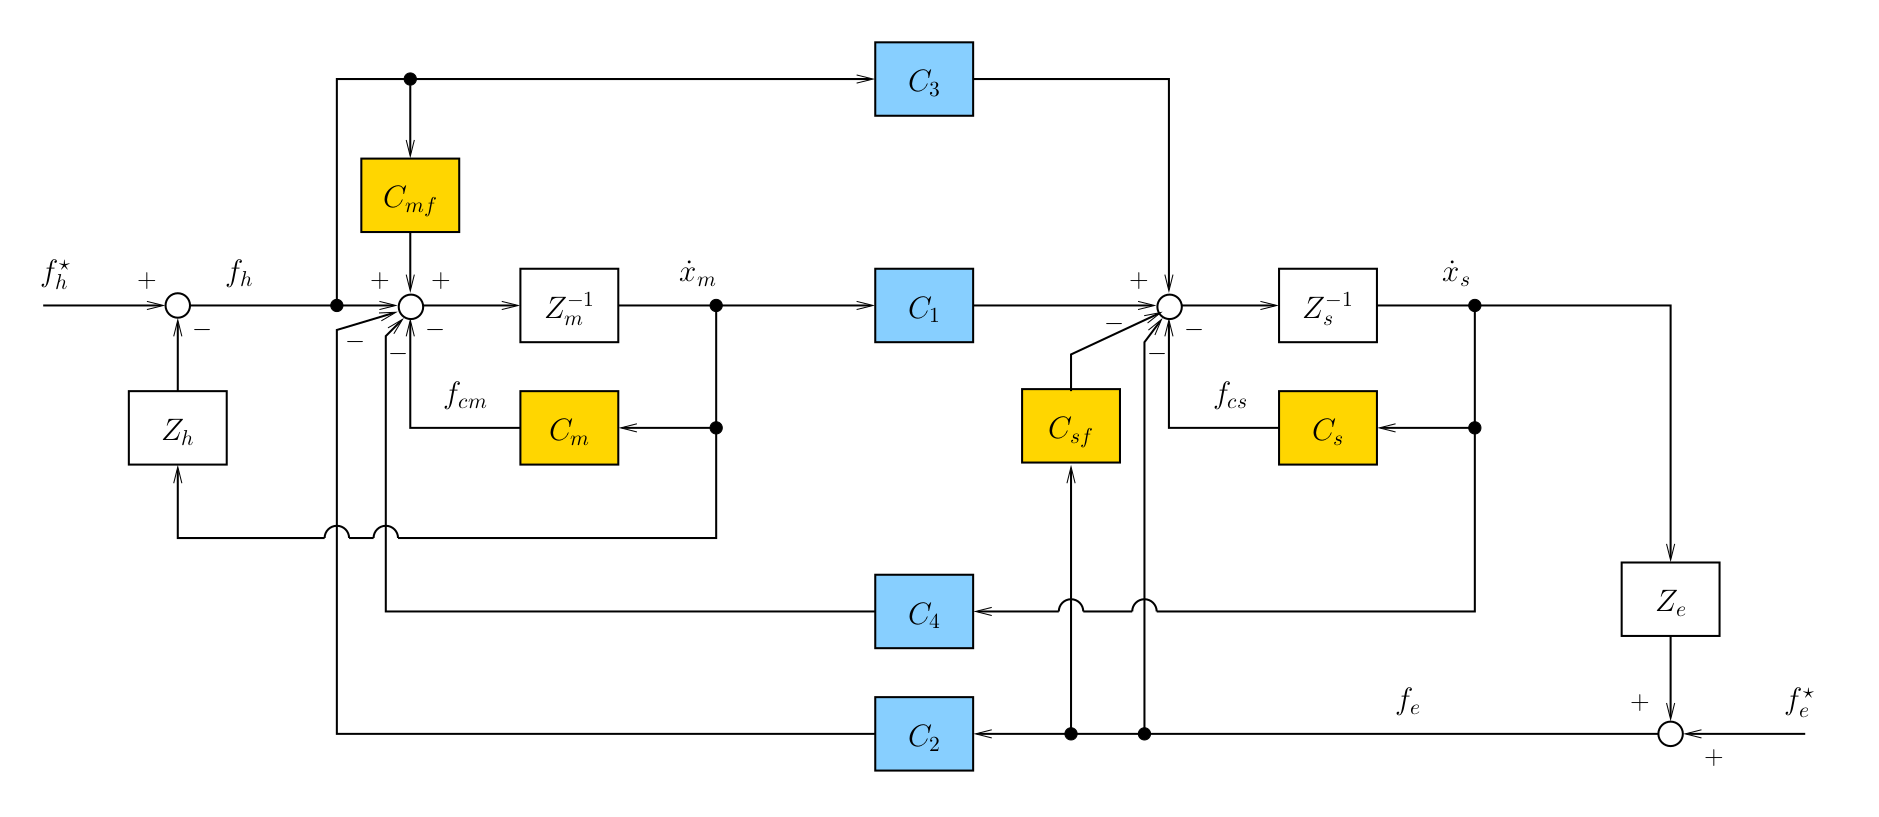
\includegraphics[scale=0.3]{images/four_channel.png}
    \end{center}
    \caption{4 Channel Bilateral Telemanipulation architecture with inner force loops $C_{mf}$ and $C_{sf}$.}
    \label{fig:four_channel}
\end{figure}

\subsection{HW 1: Continuous and discretized implementation}
Implement the SISO Four-channel bilateral teleoperation architecture with
\[
    C_m = B_m + \frac{K_m}{s} \quad
    C_s = B_s + \frac{K_s}{s}
\]
\[
    Z_m^{-1} = \frac{1}{M_ms + D_m} \quad
    Z_s^{-1} = \frac{1}{M_ss + D_s}
\]

\bigskip
\noindent where $Mm = 0.5$, $M_s = 2$. Moreover $D_s = 10$ and $D_m = 5$ or both zero in the initial case. In Fig \ref{fig:four_free} a simple plot of the positions and velocities (slave and master) are reported for proper selected tuning parameters of the related master and slave controller. In order to properly tune the controllers the following closed-loop systems were considered:

\[
G_m = \frac{1}{M_ms^2+B_ms+K_m} \quad
G_s = \frac{1}{M_ss^2+B_ss+K_s}
\]

\begin{figure}[H]
    \begin{center}
        \hspace*{-4.2cm}
        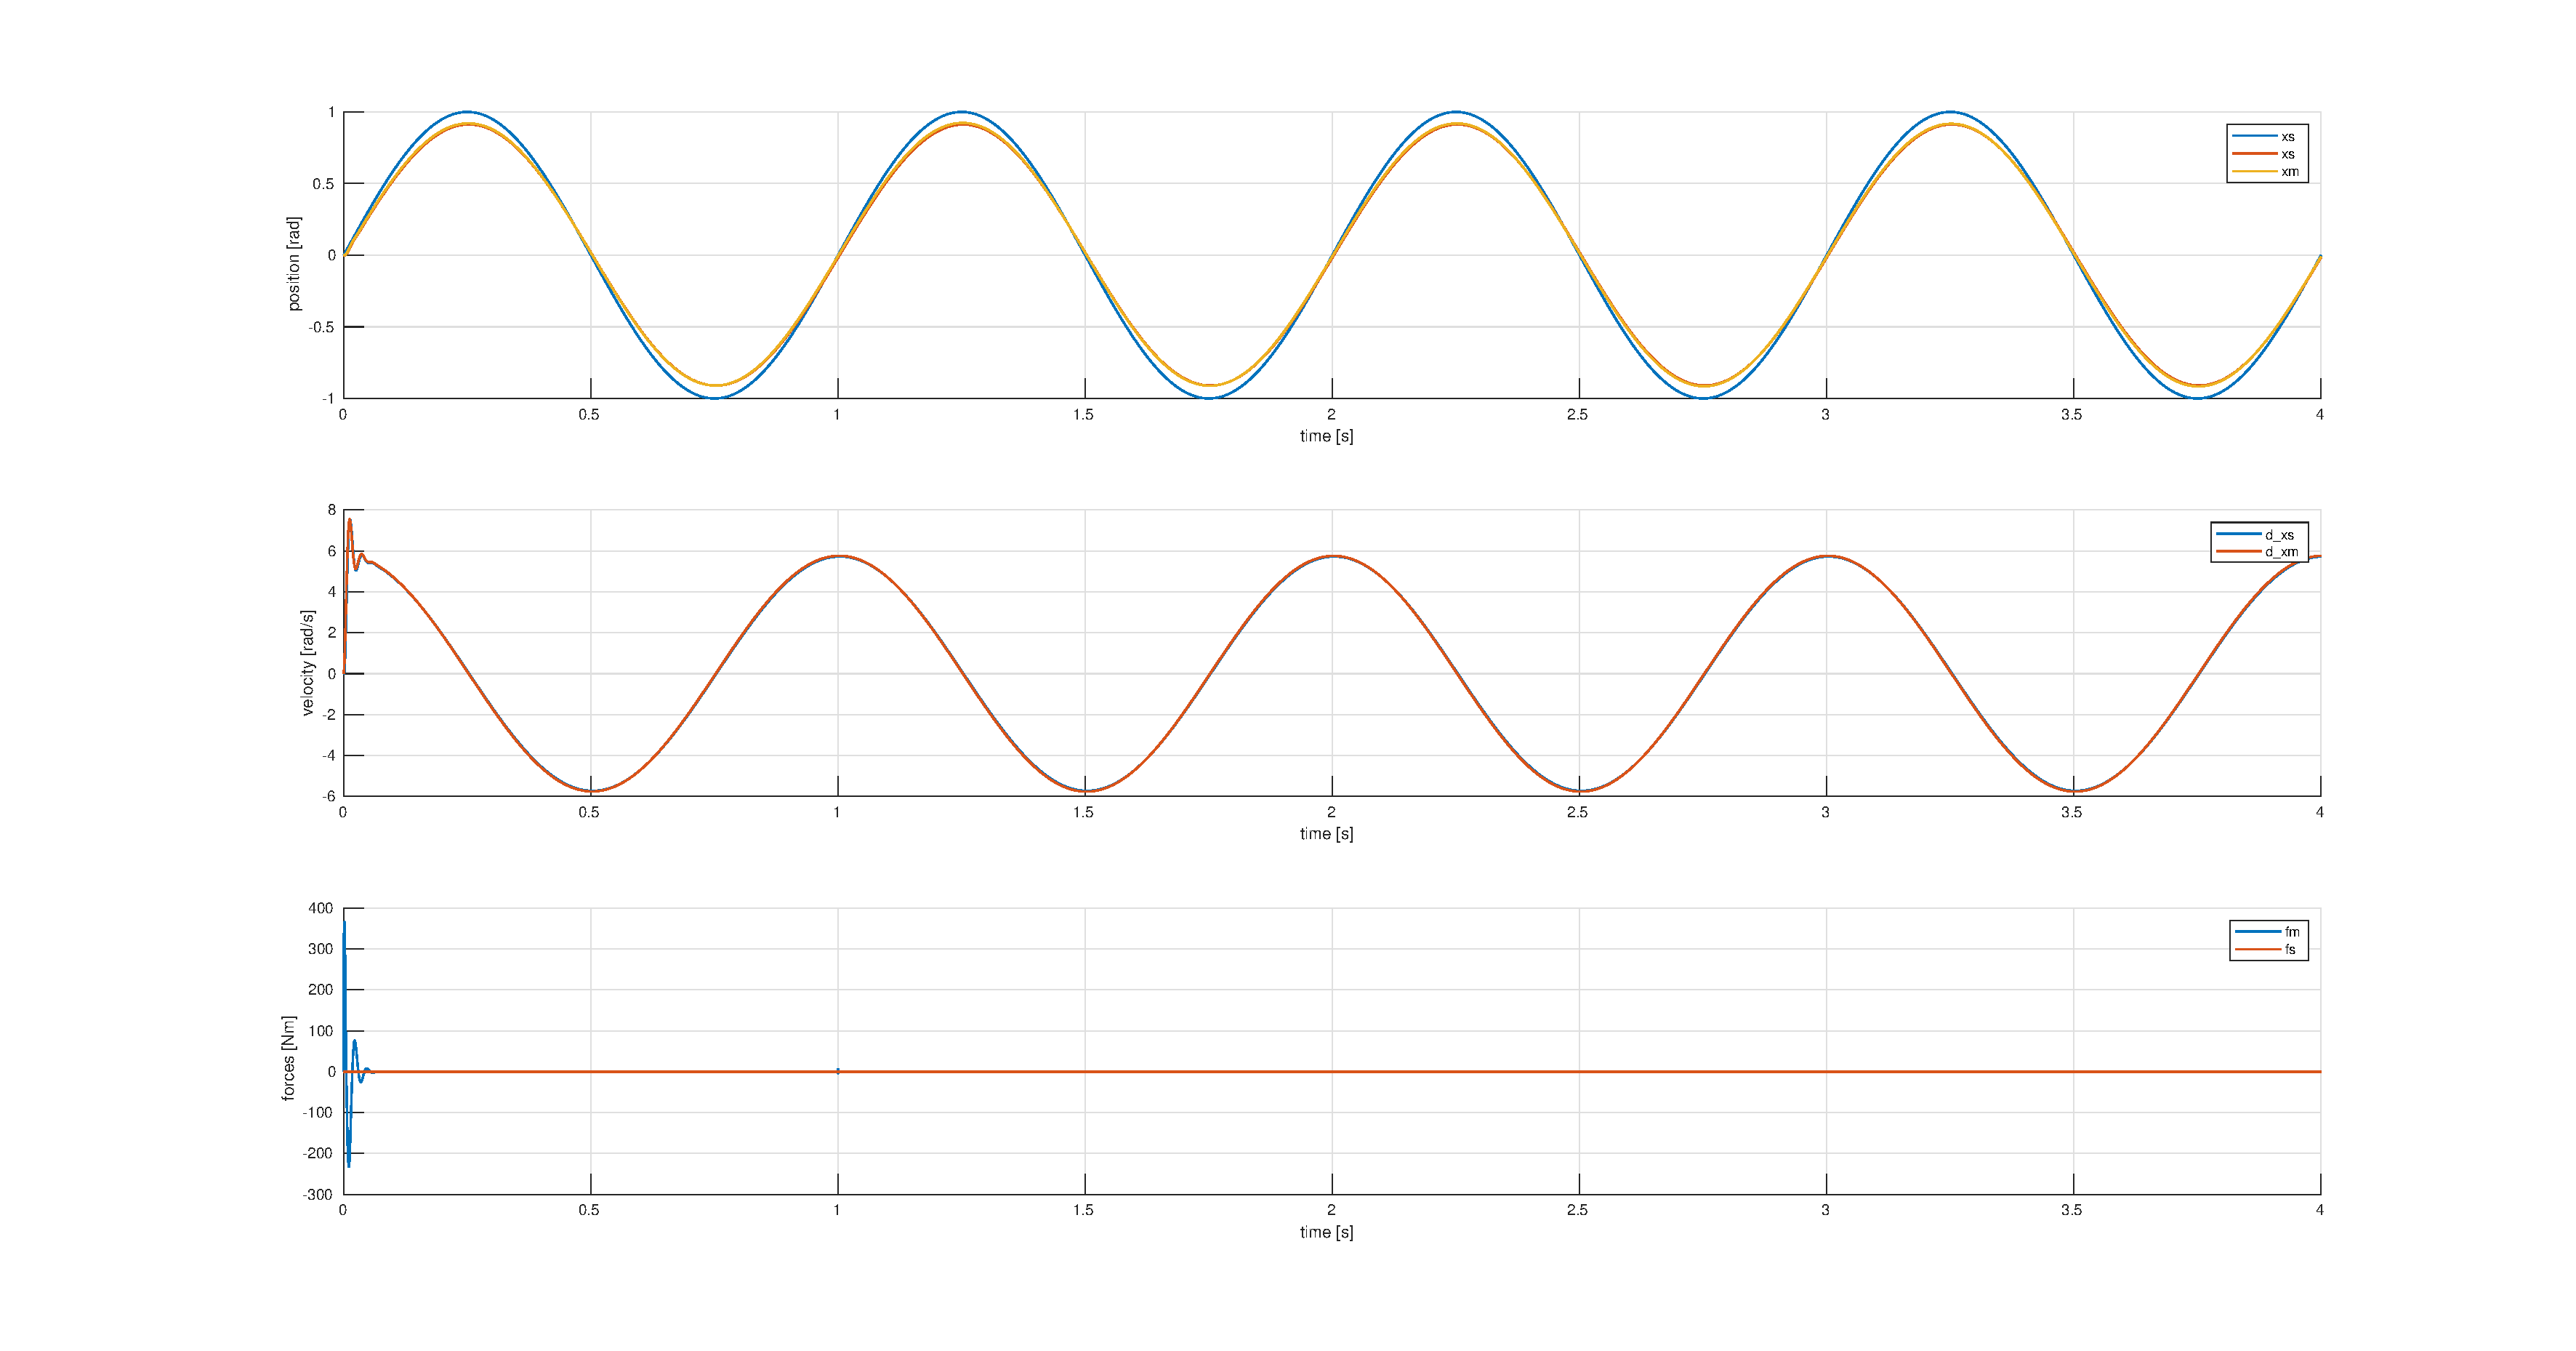
\includegraphics[scale=0.4]{images/four_free_motion.eps}
    \end{center}
    \caption{4 channel architecture in free motion with a sinusoidal reference}
    \label{fig:four_free}
\end{figure}

\bigskip
\noindent The proper parameters were selected considering the step reponse of the two second order systems. For the human intention controller the parameters were selected by comparing the reference position with the master/slave position and perform proper tuning (an analytical closed-loop system might also be considered for this analysis).
\bigskip 

\begin{figure}[H]
    \begin{center}
        \hspace*{-4.2cm}
        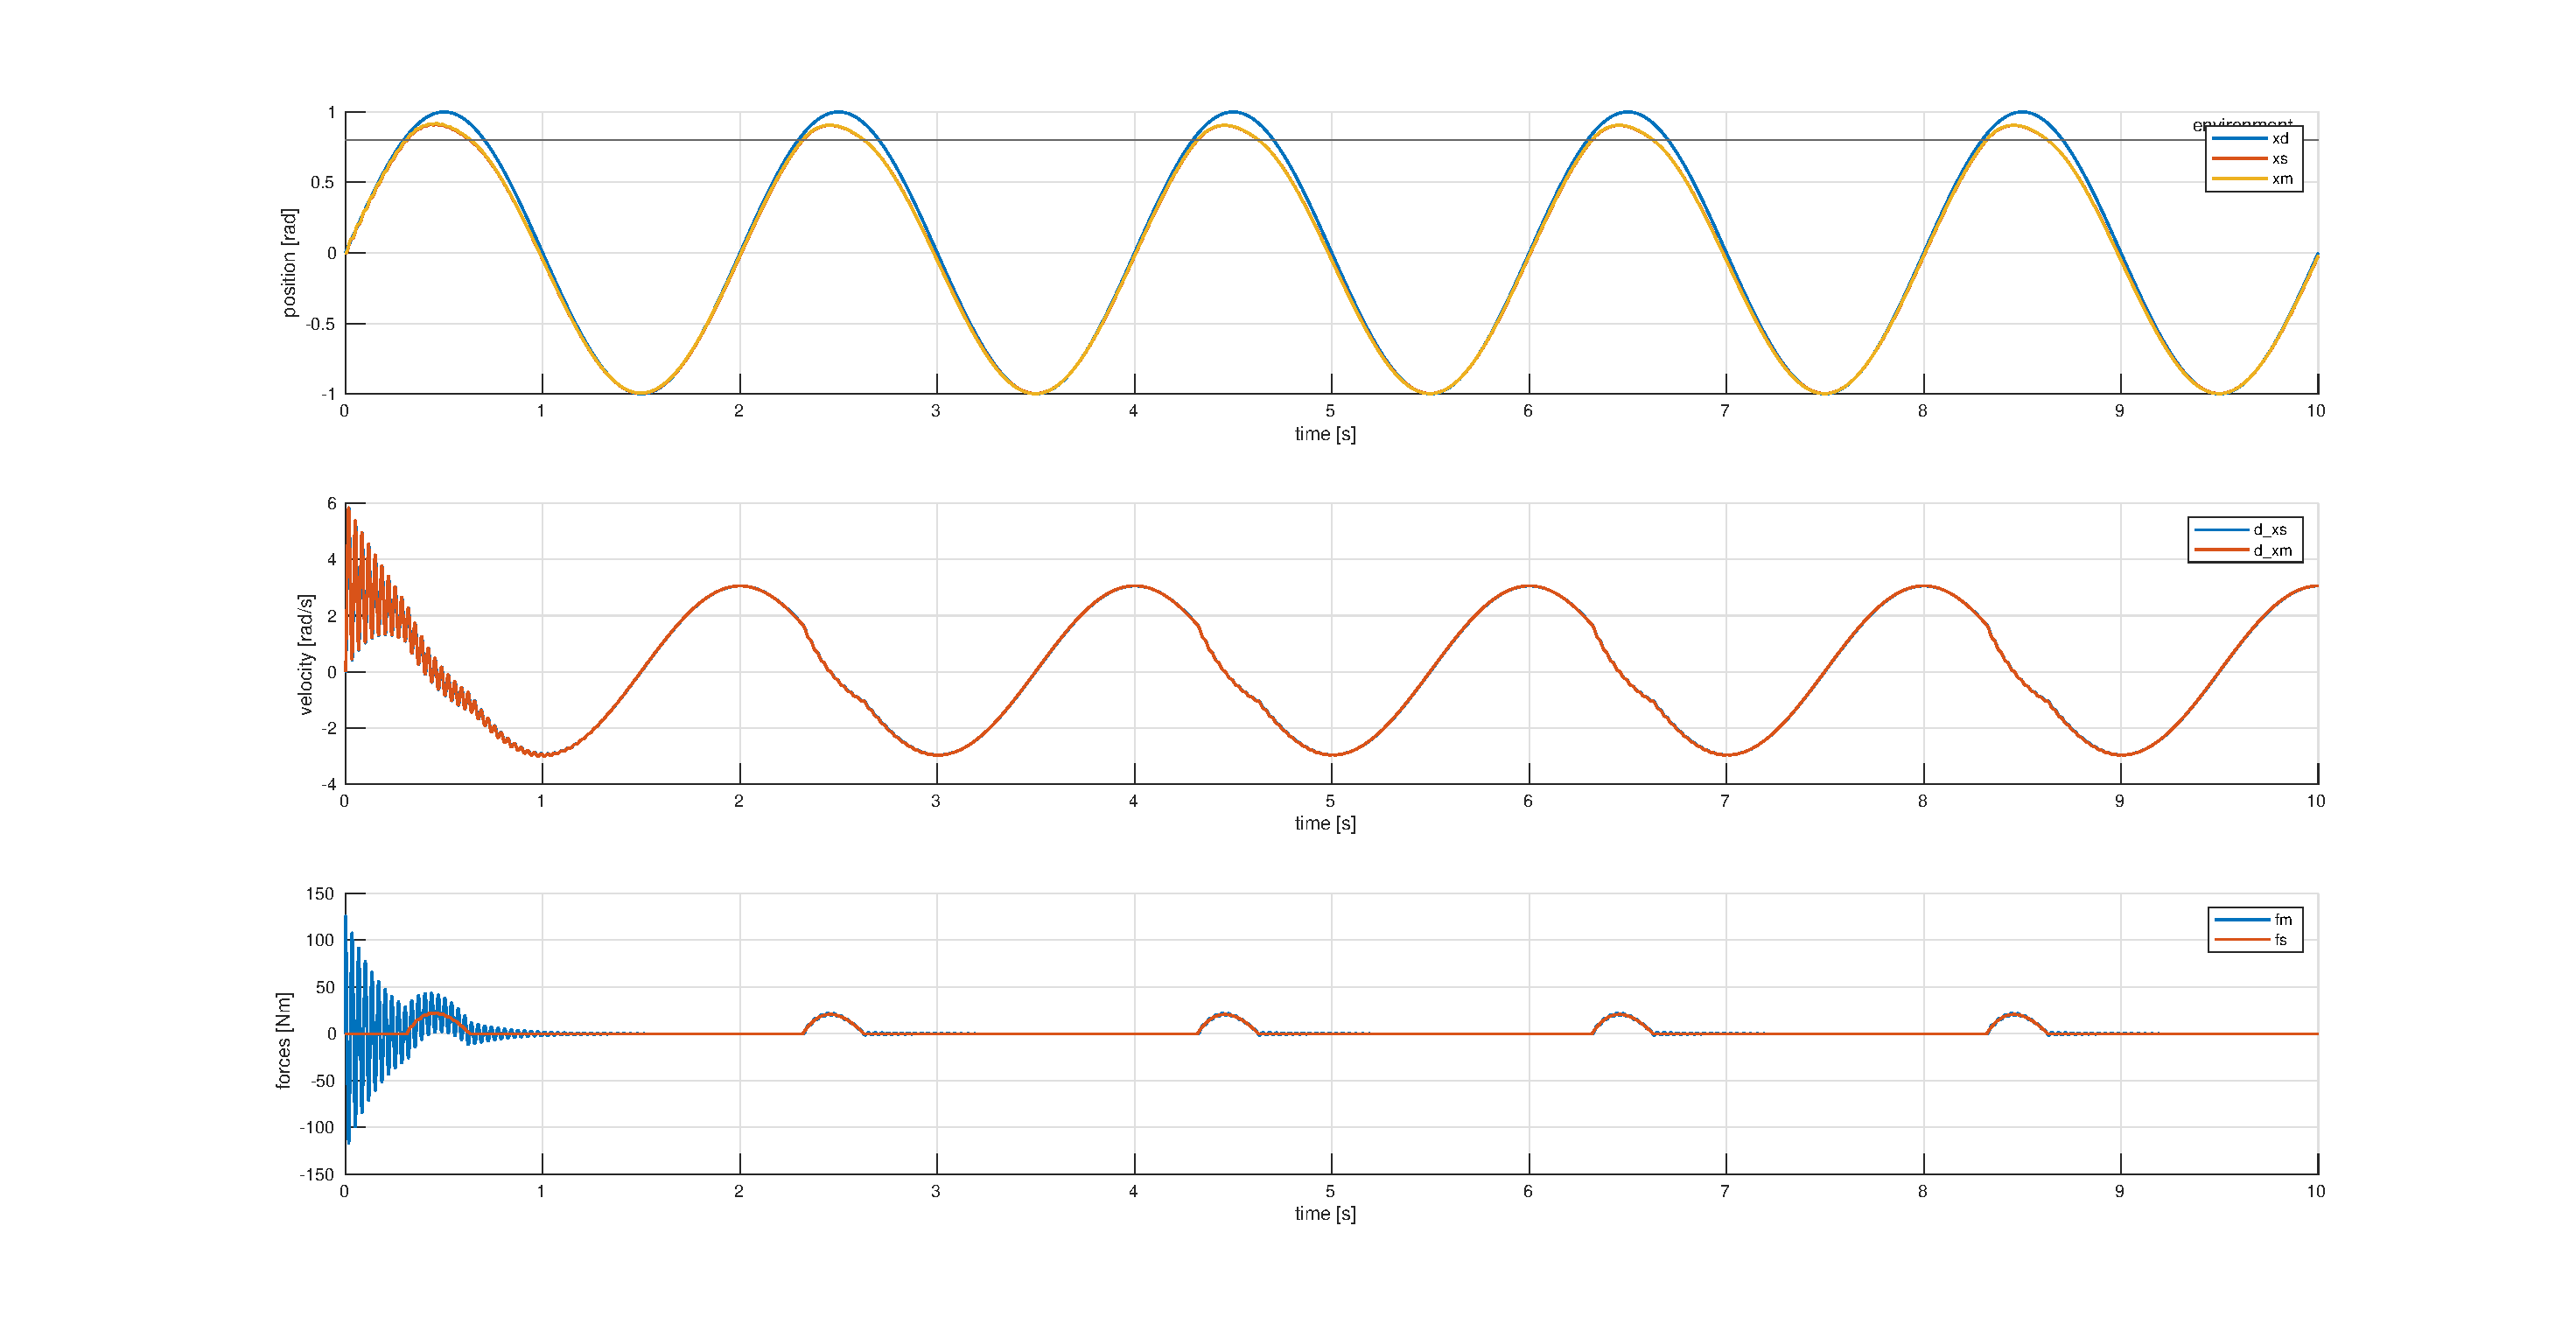
\includegraphics[scale=0.4]{images/four_contact_05.eps}
    \end{center}
    \caption{4 channel architecture in contact at 0.5 with a sinusoidal reference}
    \label{fig:four_cotact}
\end{figure}

\begin{figure}[H]
    \begin{center}
        \hspace*{-4.2cm}
        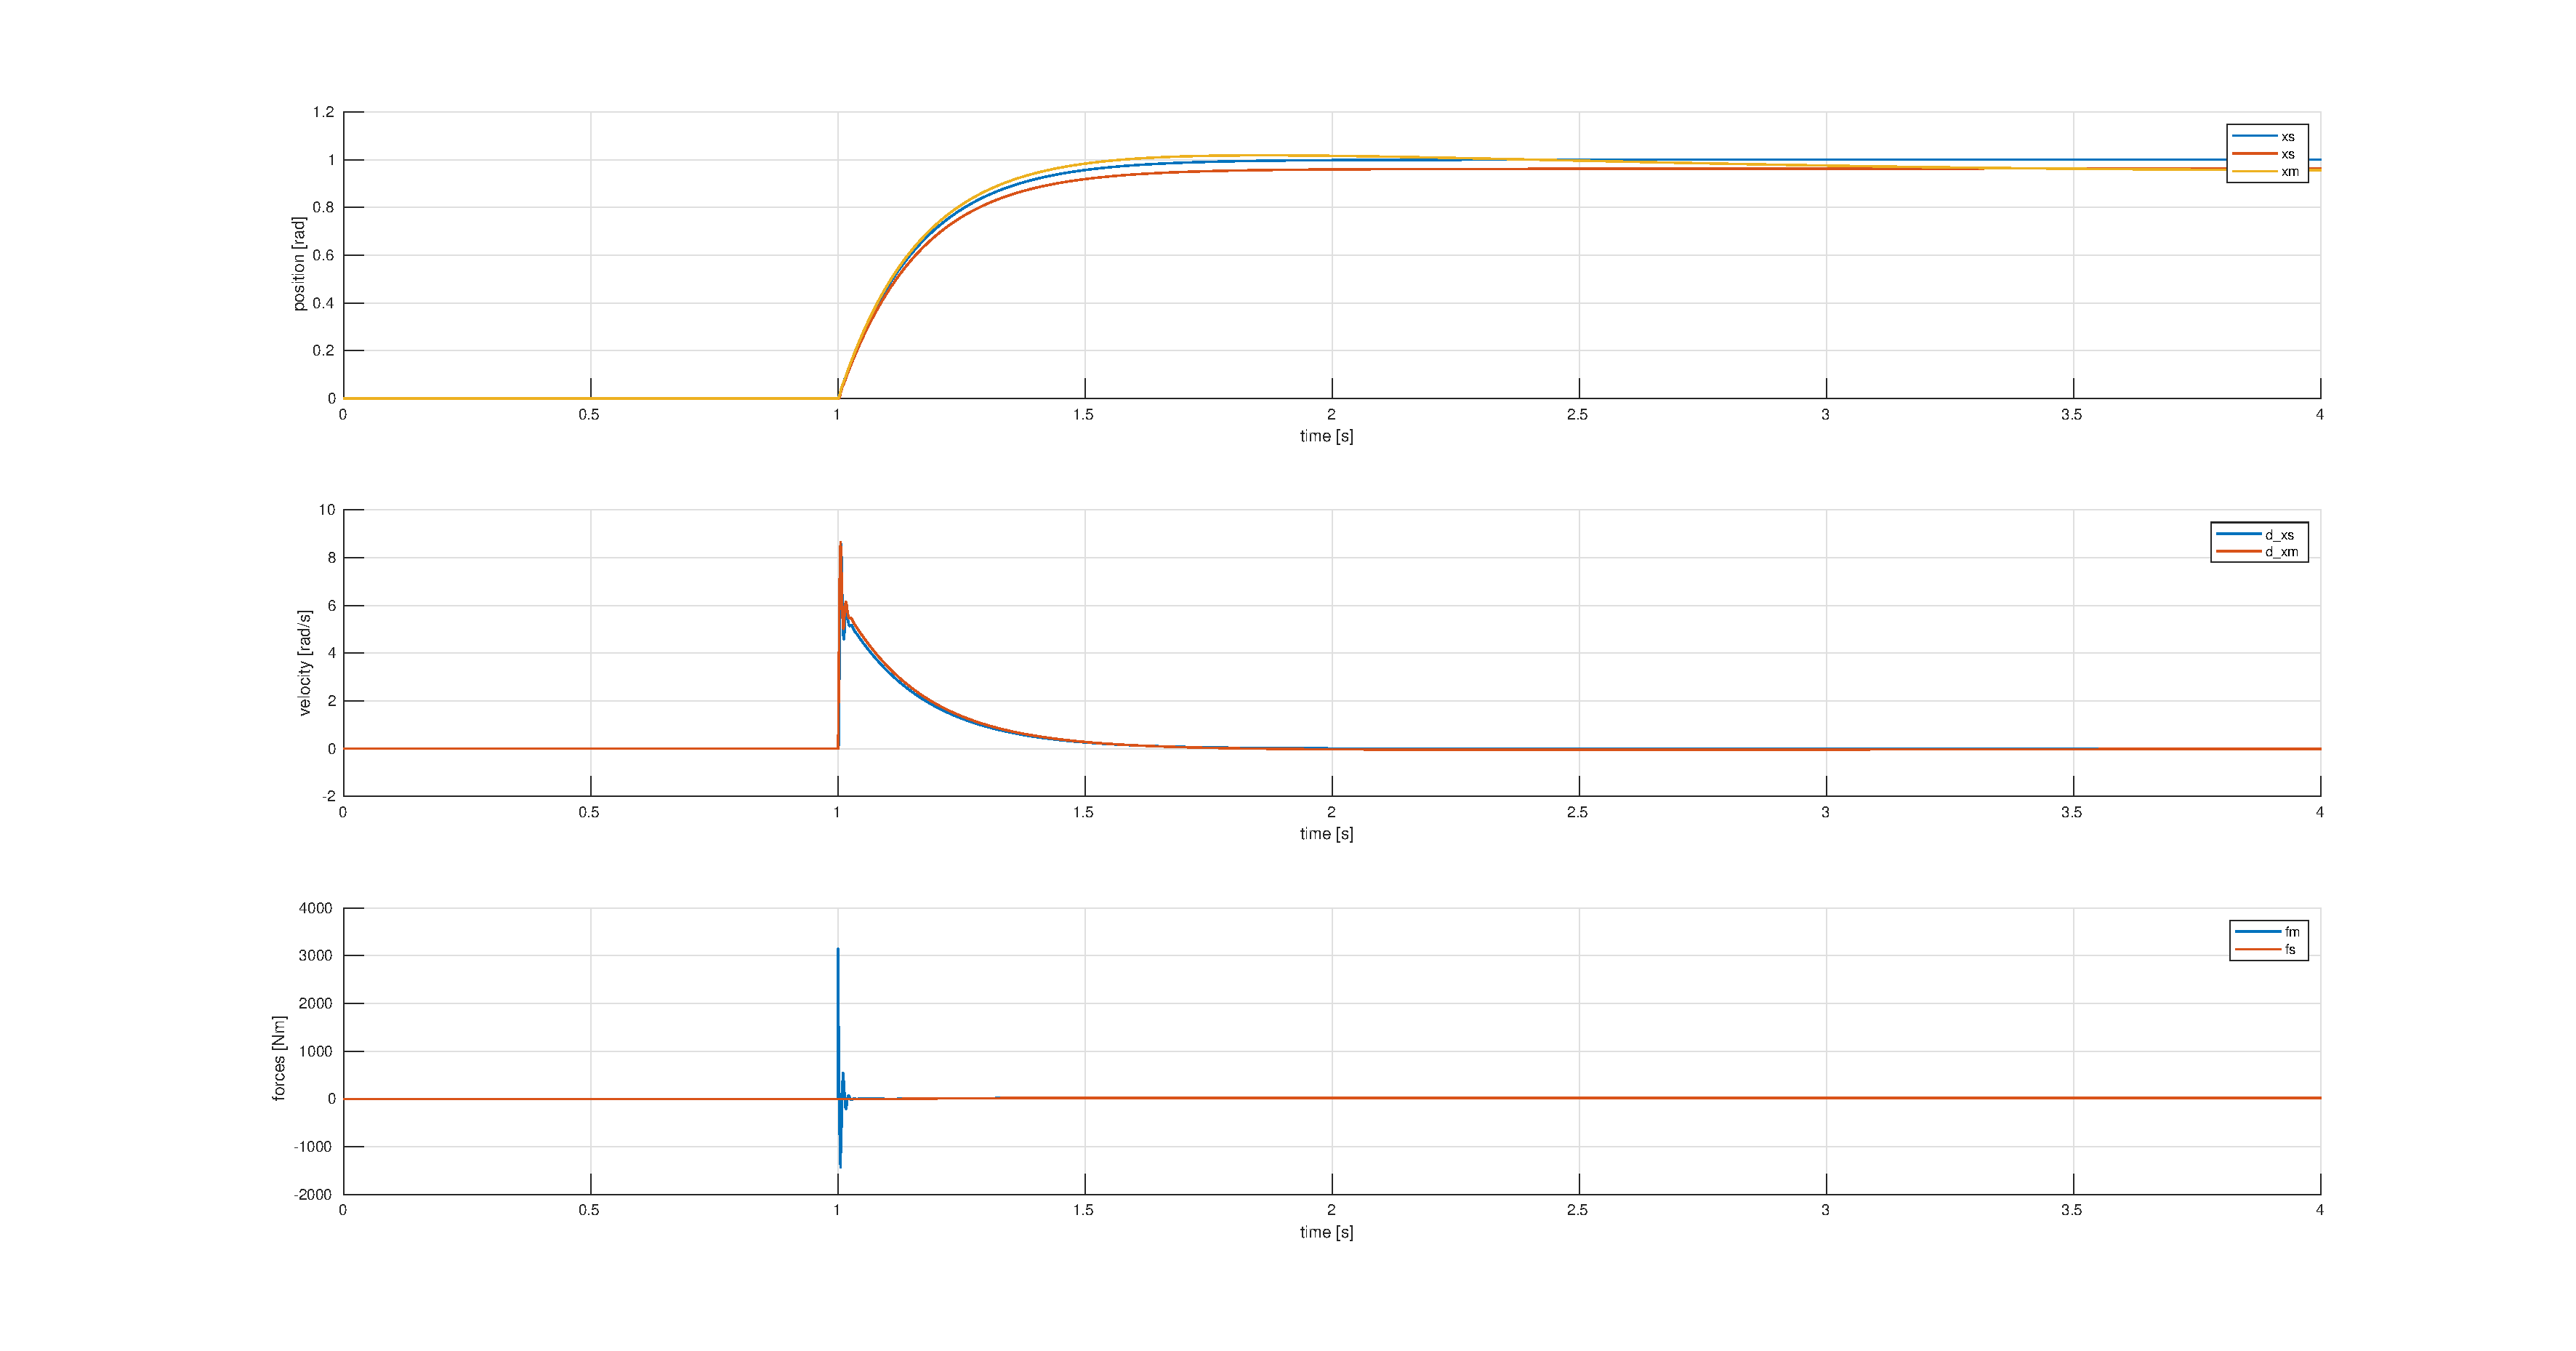
\includegraphics[scale=0.4]{images/four_step_contact_05.eps}
    \end{center}
    \caption{4 channel architecture in contact at 0.5 with a step reference}
    \label{fig:four_step}
\end{figure}

As it is visible in Fig \ref{fig:four_free} the architecture is correctly following the reference provided. There is however a large effect due to the initial motion in all the presented figures due to high gain. In Fig \ref{fig:four_cotact} the contact interaction is clearly visible in the forces plot when the position reaches 0.5. 

Finally the Fig \ref{fig:four_step} gives an idea of the reponse of the system to a step function and Fig \ref{fig:four_noisy} emphasises the problem related to estimation of velocity and accelerations with noisy measurements. Moreover the inner force feedback can be introduced as constants and be properly tuned as desired.

\begin{figure}[H]
    \begin{center}
        \hspace*{-4.2cm}
        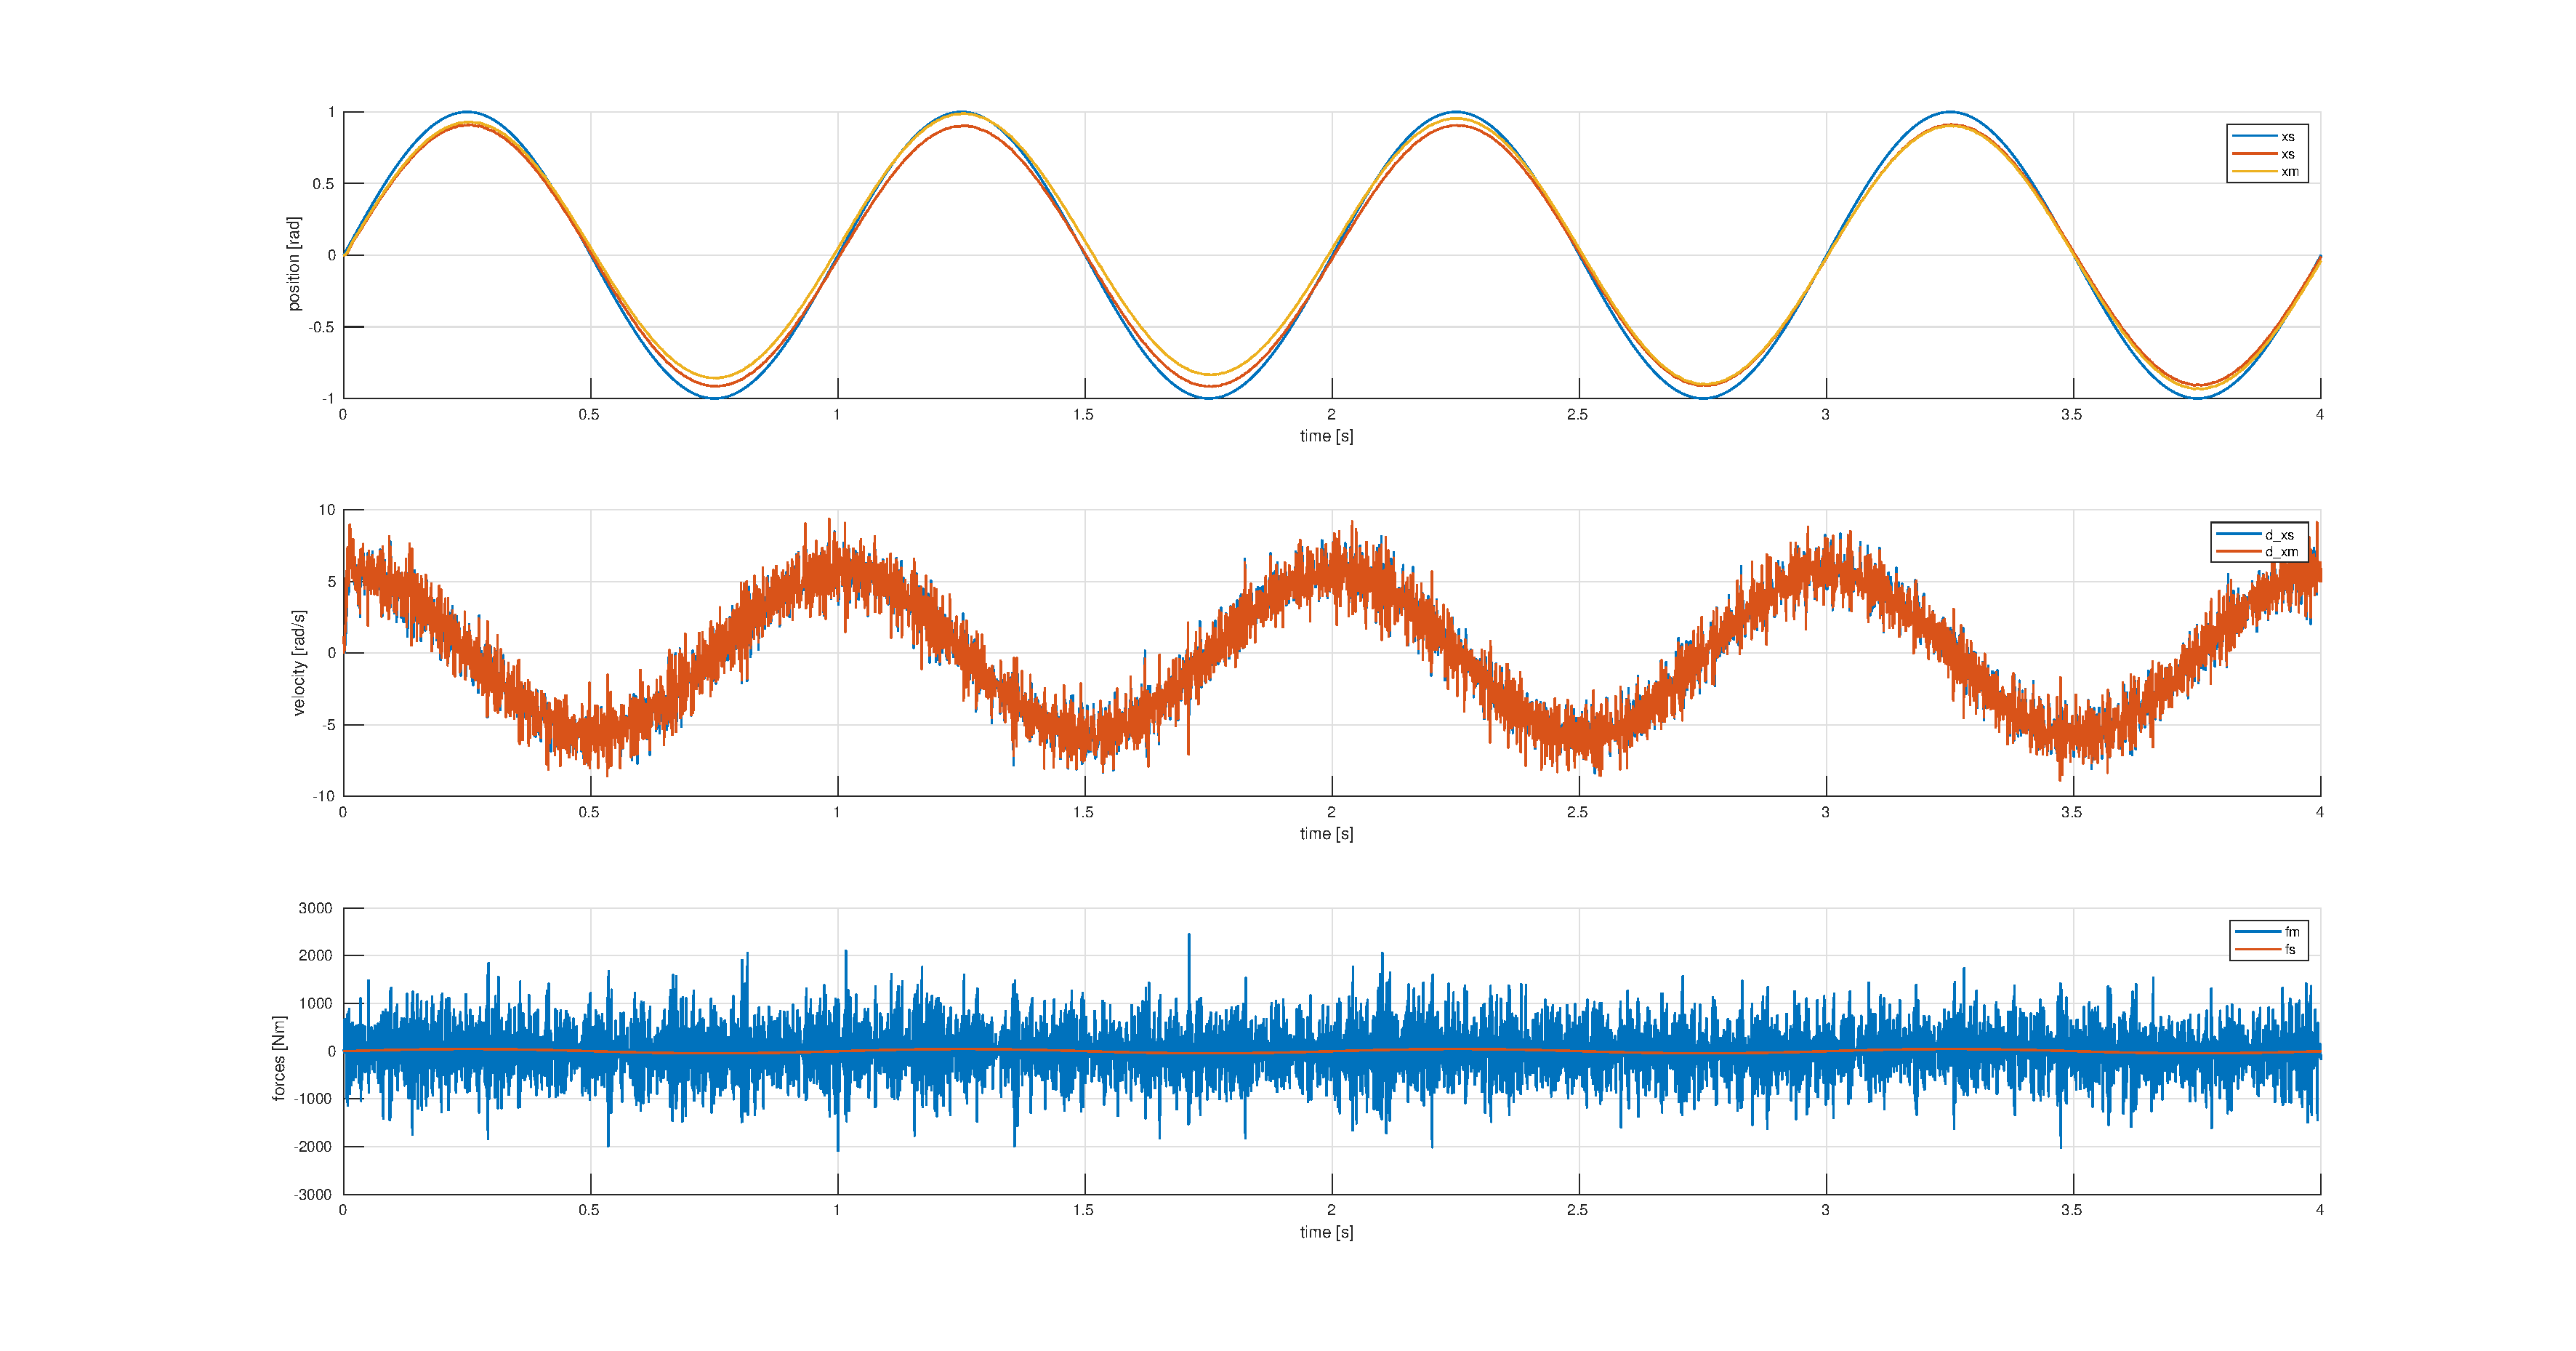
\includegraphics[scale=0.4]{images/four_noisy.eps}
    \end{center}
    \caption{Four channel architecture with white noise}
    \label{fig:four_noisy}
\end{figure}

\noindent The entire architecture was translated in the related discretized version according to our specification in terms of encoders and the related derivative were performed using the simulink block. In the following section kalman filters will be introduced and they will be used to filter noisy estimations of velocities and accelerations.

\subsection{HW 2: Derive hybrid matrix}

Derive the hybrid matrix for the four channel bilateral teleoperation considering the inner force loop at the master and slave side. We can directly consider Fig \ref{fig:four_channel}.

\[
\begin{bmatrix}  f_m \\ -v_s \end{bmatrix} = \begin{bmatrix}
    \overline{H_{11}} & \overline{H_{12}} \\
    \overline{H_{21}} &  \overline{H_{22}} \\
\end{bmatrix} = \begin{bmatrix}  v_m \\ f_s \end{bmatrix}
\]

\noindent Let's start by defining:
\begin{equation}
    v_m = Z_{cm}^{-1}(f_m -C_2f_s-C_4v_s+C_{mf}f_m)
\end{equation}
\begin{equation}
    v_s = Z_{cs}^{-1}(-f_s -C_{sf}f_s+C_1v_m+C_3f_m)
\end{equation}

\noindent Finally let's compute the 4 components of the hybrid matrix considering one component to zero at each step.
\[
    \overline{H_{11}} : f_m \rightarrow v_m \qquad f_s = 0
    \]\[
    Z_{cm}v_m = f_m - C_4Z_{cs}^{-1}C_1v_m - C_4Z_{cs}^{-1}C_3f_m + C_{mf}f_m
\]\[
    v_m(Z_{cm}+C_4Z_{cs}^{-1}C_1) = f_m(1-C_4Z_{cs}^{-1}C_3 + C_{mf})
    \]\[
    \overline{H_{11}} = \frac{Z_{cm}Z_{cs}+C_1C_4}{(1+C_{mf})Z_{cs} - C_3C_4}
\]


\bigskip

\[
    \overline{H_{12}} : f_m \rightarrow f_s \qquad v_m = 0
    \]\[
    0 = f_m -C_2f_s +C_4Z_{cs}^{-1}C_{sf}f_s + C_4Z_{cs}^{-1}f_s - C_{mf}f_m
\]\[
    f_m(1-C_{mf}-C_4Z_{cs}^{-1}C_3) = f_s(C_2-C_4Z_{cs}^{-1}C_{sf}C_{sf}-C_4Z_{cs}^{-1})
    \]\[
    \overline{H_{12}} = \frac{C_2Z_{cs}-C_4(1+C_{sf})}{(1+C_{mf})Z_{cs} - C_3C_4}
\]

\bigskip

\[
    \overline{H_{21}} : -v_s \rightarrow v_m \qquad f_s = 0
    \]\[
    v_sZ_{cs} = -(C_1v_m + C_3f_m)
\]\[
    v_s(Z_{cs} - \frac{C_3C_4}{1+C_{mf}} = -v_m(C_1 + \frac{C_3Z_{cm}}{1+C_{mf}})
    \]\[
    \overline{H_{21}} = -\frac{C_1(1+C_{mf}) + C_3Z_{cm}}{(1+C_{mf})Z_{cs} - C_3C_4}
\]


\bigskip

\[
    \overline{H_{22}} : -v_s \rightarrow f_s \qquad v_m = 0
\]\[
    v_sZ_{cs} = C_{sf}f_s + f_s + C_{sf}f_s
\]\[
    v_s(Z_{cs}-\frac{C_3C_4}{1+C_{mf}}) = f_s(C_{sf} + 1 - \frac{C_3C_2}{1+C_{mf}})
\]\[
    \overline{H_{22}} = \frac{(1+C_{sf})(1+C_{mf})-C_2C_3}{(1+C_{mf})Z_{cs}-C_3C_4}
\]

\section{HW 3-4: Kalman Filter, Predictor and Smoother}
In this section we are briefy going to consider the following estimation problems:
\begin{itemize}
    \item \textbf{Filtering} estimate $\hat{s}(t)$ using measurements till time t
    \item \textbf{Prediction}: estimate $\hat{s}(t+h)$ using measurements till time t
    \item \textbf{Smoothing}: estimate $\hat{s}(t-h)$ using measurements till time t
\end{itemize}
\bigskip

Our aim is to estimate the velocities and accelerations from noisy position measurements. Some samples were provided for the task and the kalman filter and predictor were implemented as well as the steady state versions. The theory behind the kalman filter and predictor is not fully reported. Let's derive the discretized model for the position, velocities and accelerations to use in the kalman filter:

\begin{equation}
    \dot{x}(t) =  \begin{bmatrix}  0&1&0 \\ 0&0&1\\0&0&0 \end{bmatrix} x(t) + \begin{bmatrix}  0\\0\\1 \end{bmatrix} w(t)
    \qquad
    y(t) = \begin{bmatrix}  1&0&0 \end{bmatrix}x(t) + v(t)
\end{equation}

\noindent Let's discretize the continuous-time model:
\[
    A_d = e^{AT_s} = e^{\begin{bmatrix}  0&1&0 \\ 0&0&1\\0&0&0 \end{bmatrix}T_s} = \begin{bmatrix} 1&T_s&\frac{T_s^2}{2}\\0&1&T_s\\0&0&1 \end{bmatrix}
\]
\[
    C_d = C = \begin{bmatrix} 1&0&0 \end{bmatrix}
\]
\[
    B_d = \left (\int_{0}^{T_s} e^{\begin{bmatrix} 1&\tau&\tau^2/2\\0&1&\tau\\0&0&1 \end{bmatrix}} \,d\tau \right) = \begin{bmatrix} T_s^3/6\\T_s^2/2\\T_s \end{bmatrix}
\]

It is important to notice the presence of two variance matrixes $R$ related to $v_k$ and $Q$ related to $w_k$. The variance matrix $R$ also called noise variance depends on the sensors whereas the variance
matrix $Q$ also caled model variance is chosen in order to explain the measurements as well as
possible. They are crucial for proper tuning of the kalman filter.

\bigskip
\noindent Briefly the Kalman filter can be defined using a recursive formulation composed of a prediction and an estimation step with proper initial conditions:
\[
    \hat{x}_{k+1|k+1} = A\hat{x}_{k|K} + K_{k+1}(y_{k-1} - CA\hat{x}_{k|k})
\]   
\[
    P_{k+1|k} = AP_{k|k-1}A^T - AP_{k|k-1}C^T(CP_{k|k-1}C^T + R)^{-1}CP_{k|k-1}A^T+Q \qquad \textbf{Ricati equation}
\]

\bigskip
where the kalman gain maps the output estimation error into the correction of the prediction state
\[
    K_{k+1} = P_{k+1|k}C^T(CP_{k+1|k}C^T+R)^{-1} \qquad \textbf{Kalman gain}
\]

when k goes to infinity we can consider the steady-state kalman filter which uses the Algebraic Ricati Equation (ARE) for getting $P_{\infty}$. Informally the steady-state kalman filter is not optimal at the beginning of the experiments but we can reach reasonable results.

\begin{figure}[H]
    \begin{center}
        \hspace*{-4.6cm}
        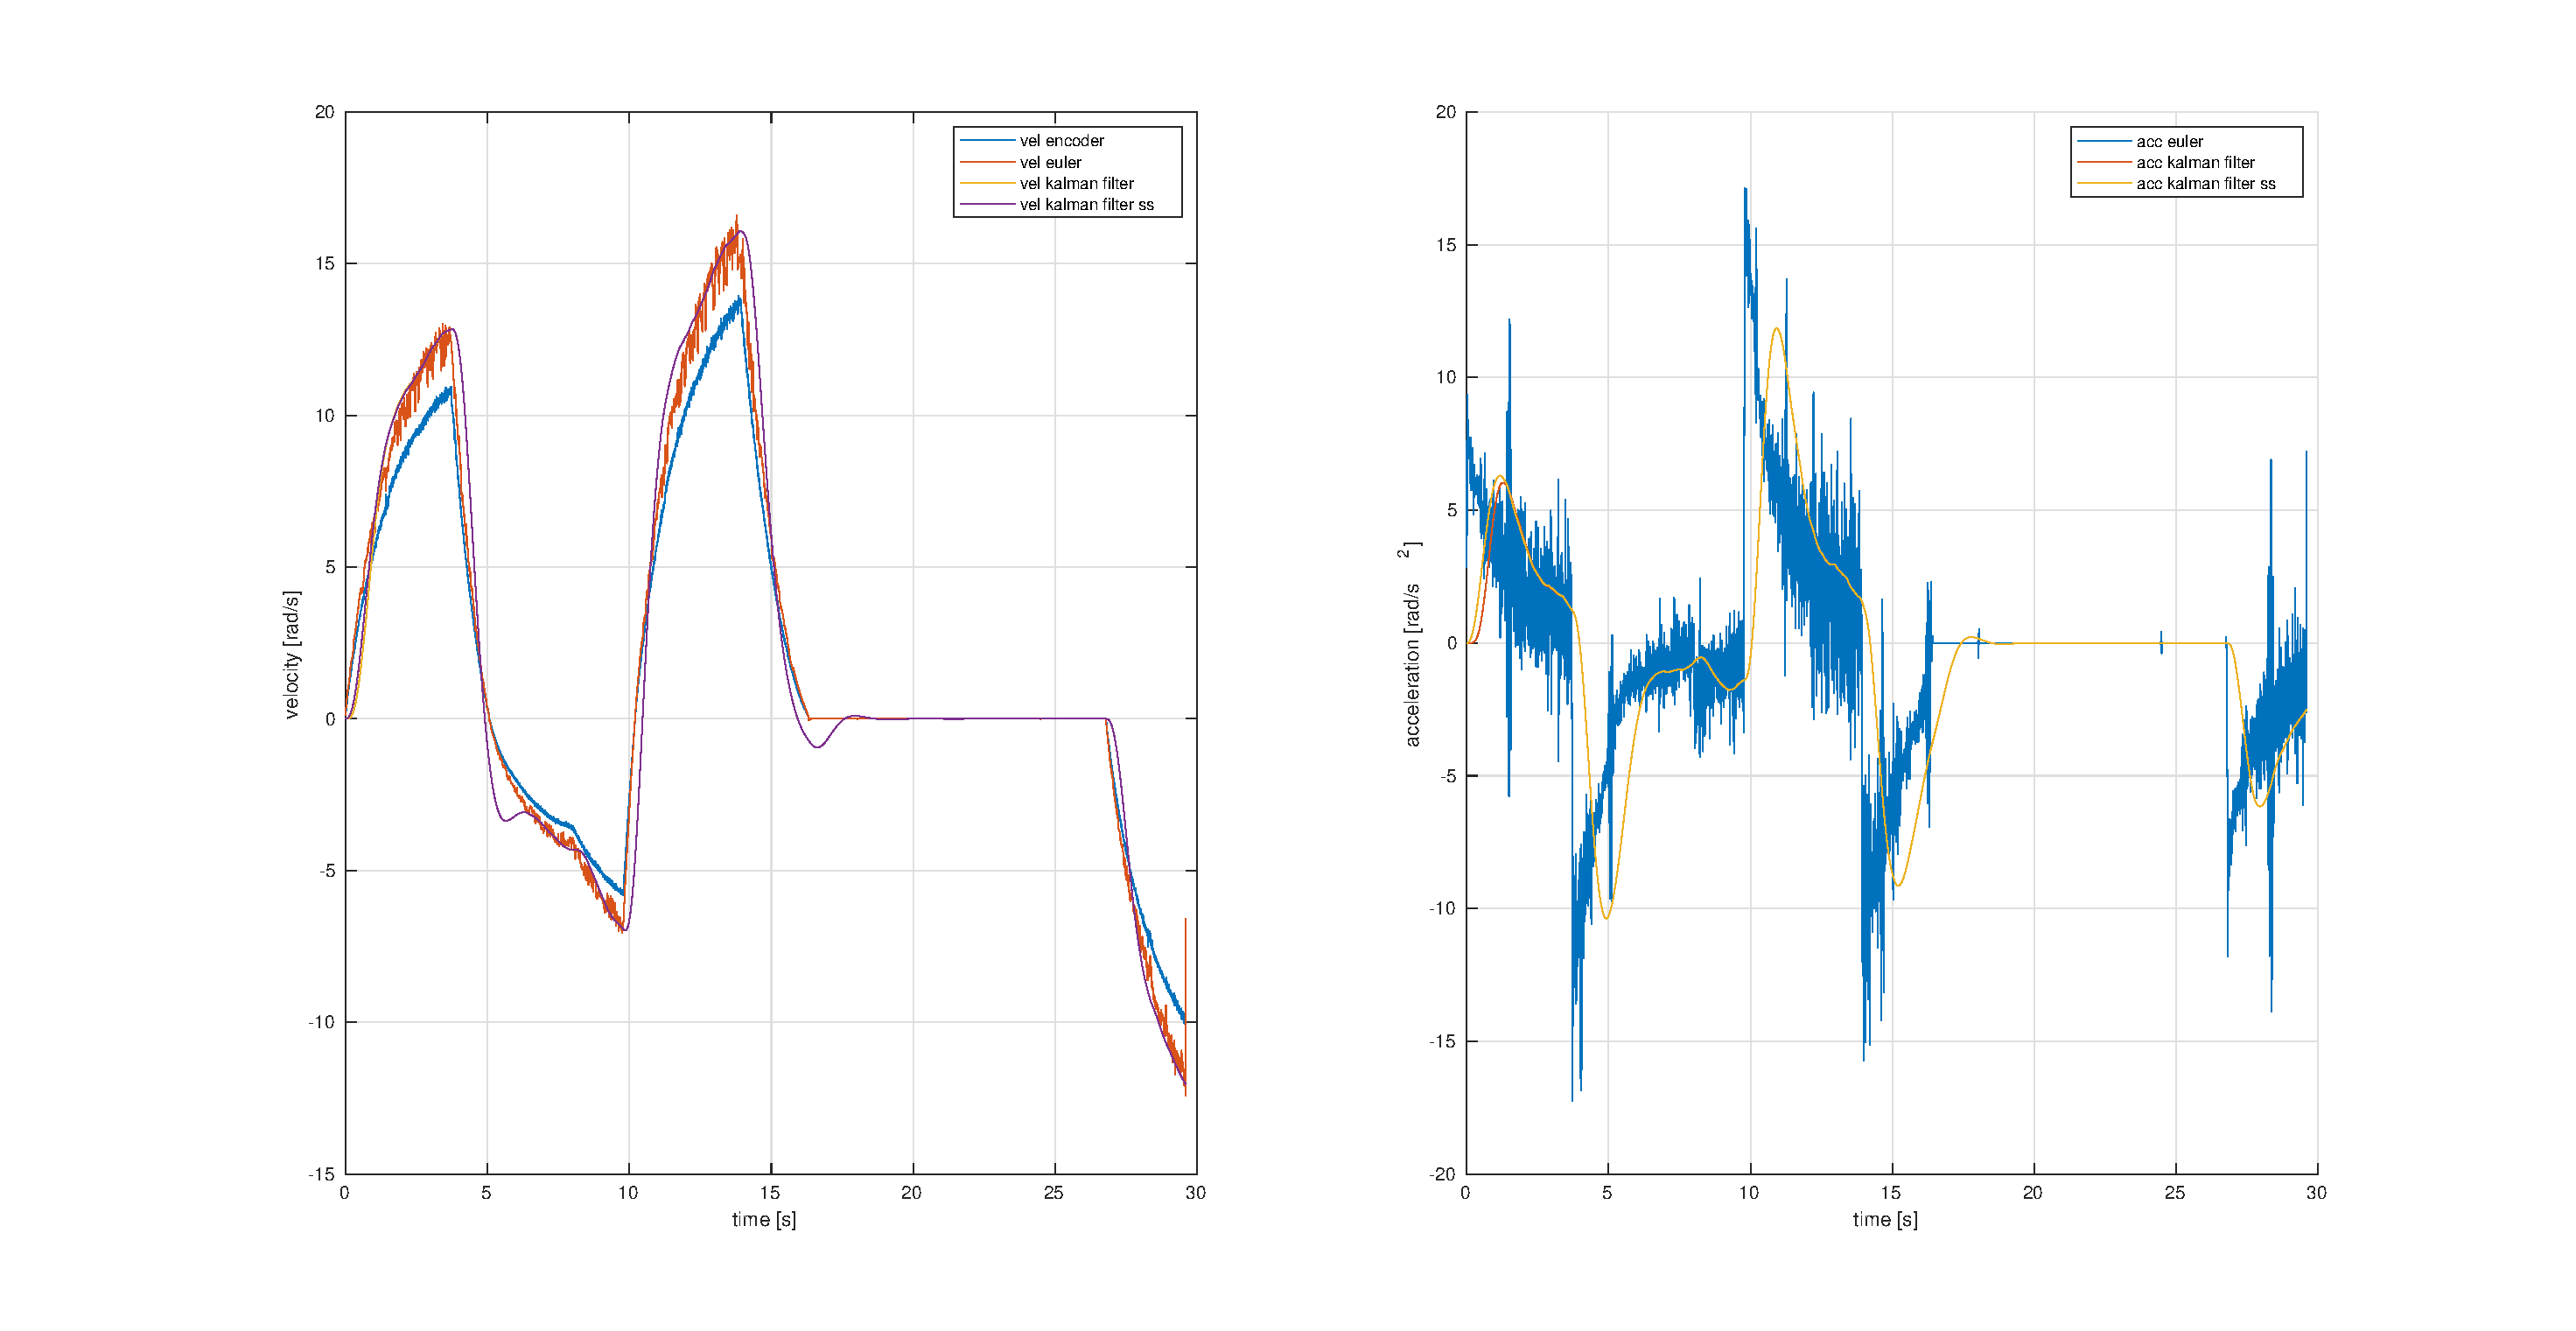
\includegraphics[scale=0.5]{images/kalman_filter.eps}
    \end{center}
    \caption{Velocities and accelerations estimations using Kalman filter, Kalman filter in steady state conditions and euler approximations with 5Hz low pass filter. As it is visible at the beginning the Kalman filter is different from the steady state version.}
    \label{fig:kalman_filter}
\end{figure}

\begin{figure}[H]
    \begin{center}
        \hspace*{-4.6cm}
        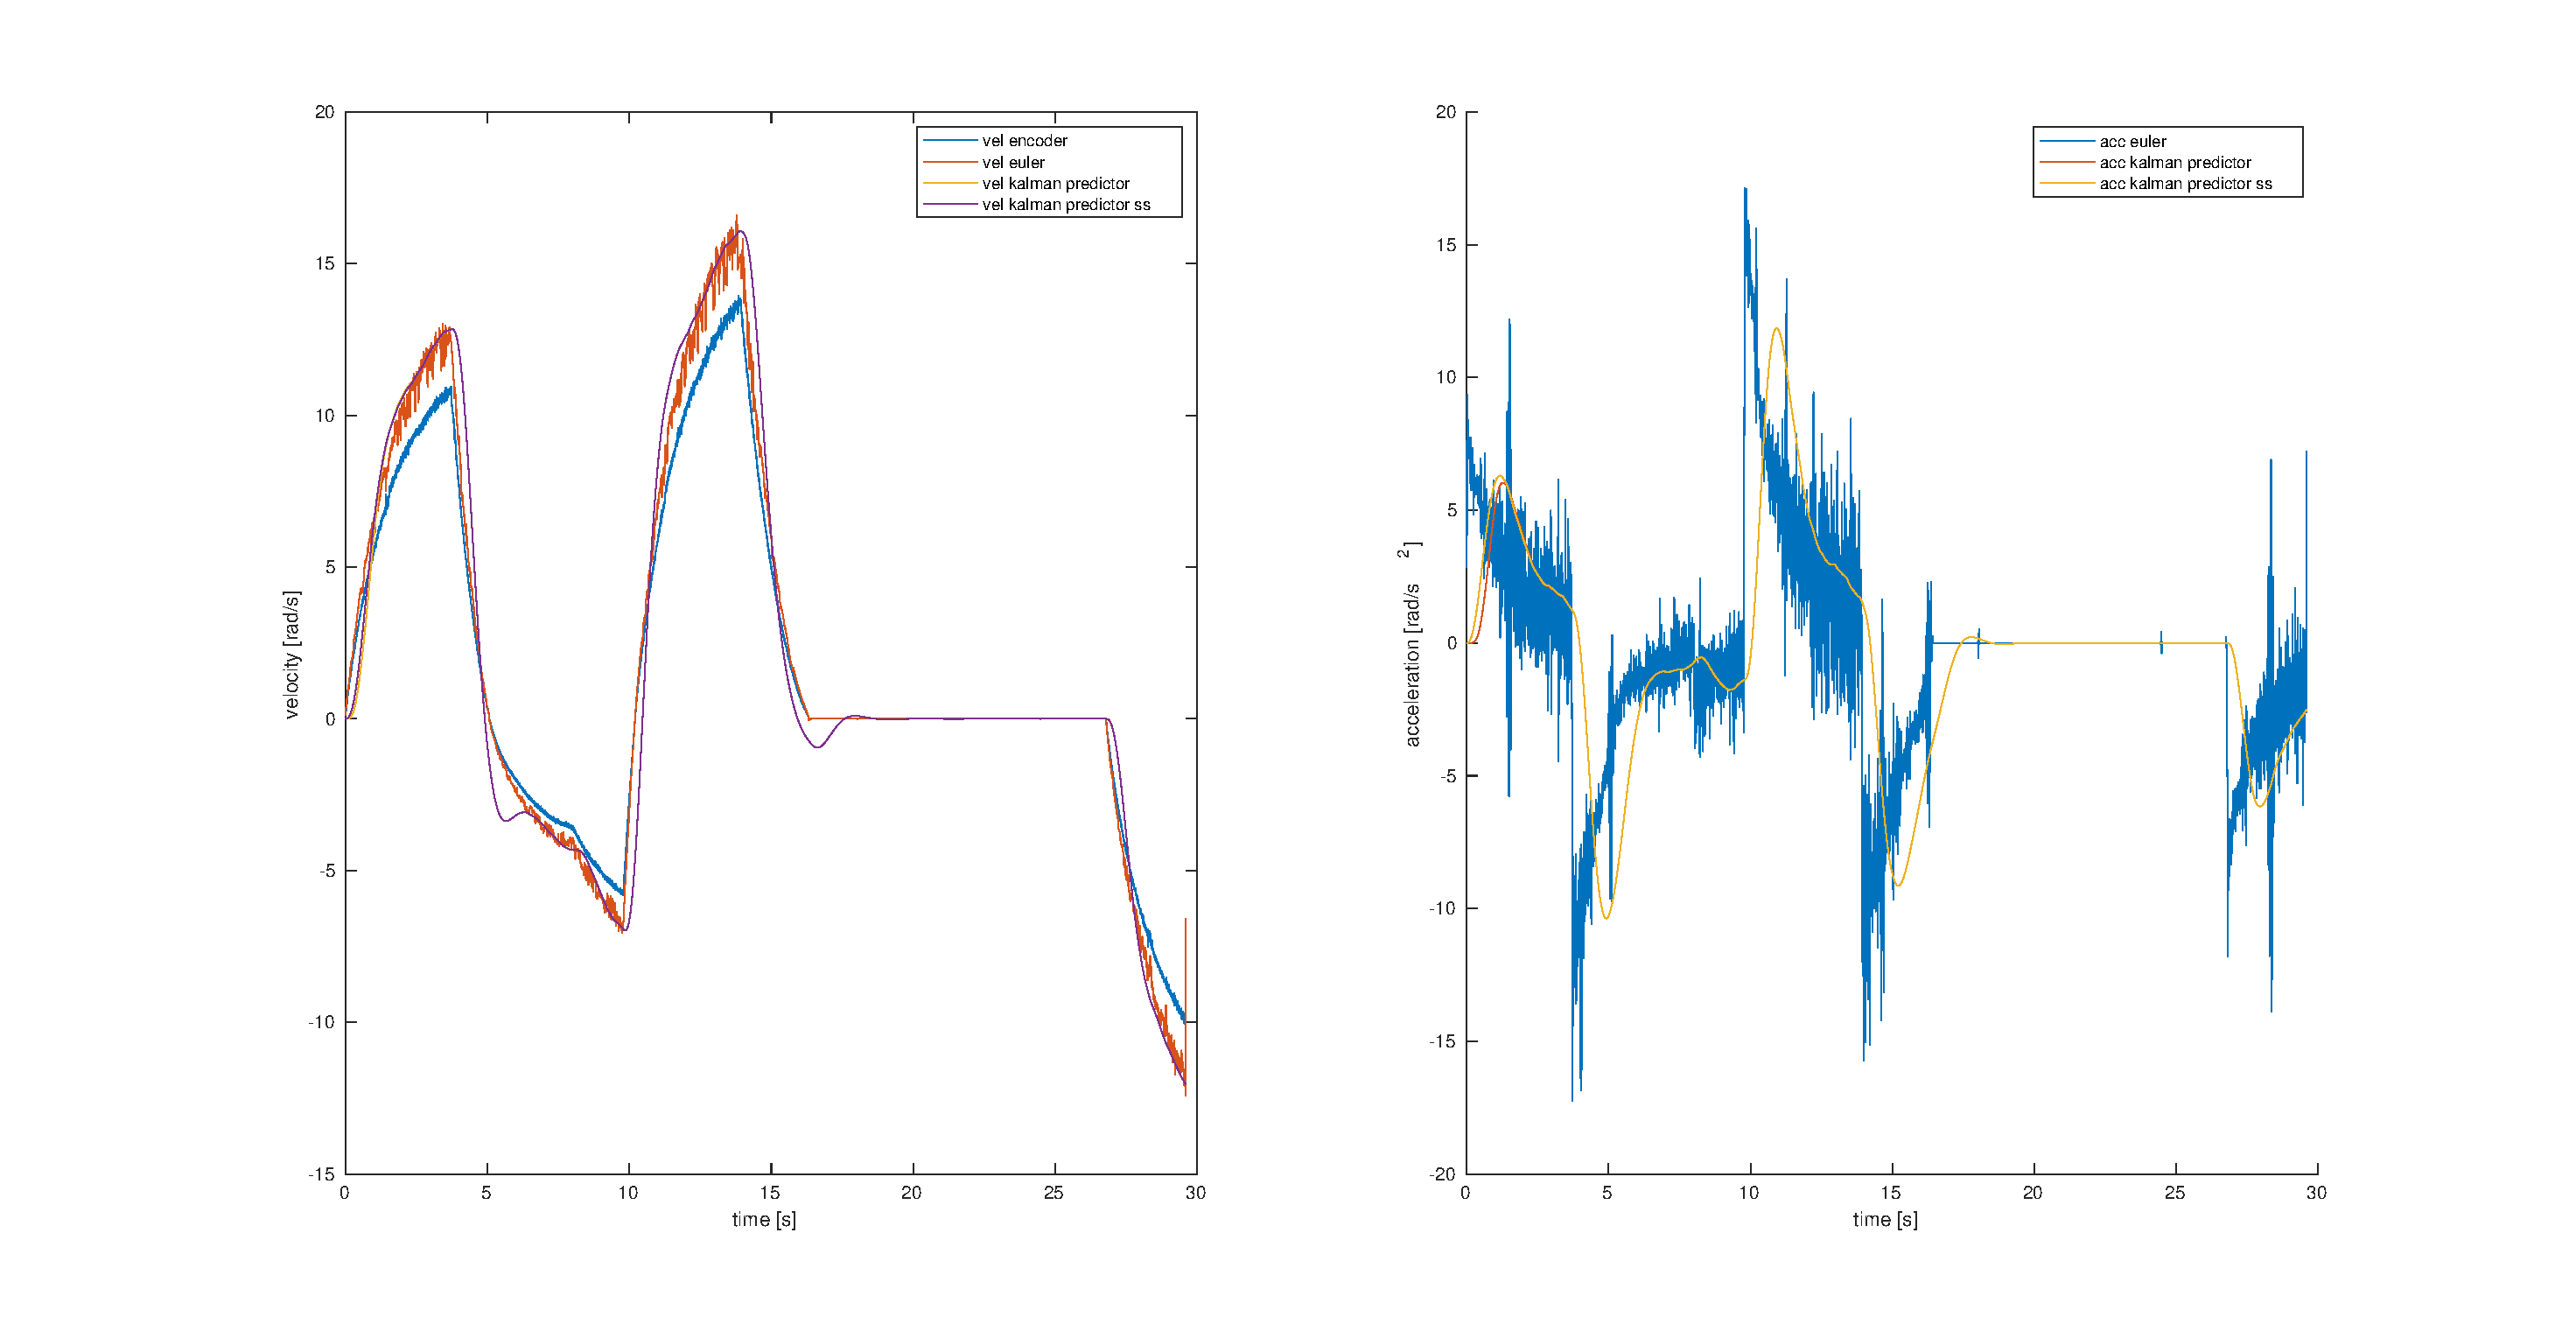
\includegraphics[scale=0.5]{images/kalman_predictor.eps}
    \end{center}
    \caption{Velocities and accelerations estimations using Kalman predictor, Kalman predictor in steady state conditions and euler approximations with 5Hz low pass filter. As it is visible at the beginning the Kalman predictor is different from the steady state version.}
    \label{fig:kalman_predictor}
\end{figure}

In Fig \ref{fig:kalman_smoother} the use of the kalman smoother is reported. Informally, thanks to both forward (Kalman filter) and backward (smoothing) steps the Kalman smoother in general performs a better estimation for the given dataset.
\begin{figure}[H]
    \begin{center}
        \hspace*{-4.6cm}
        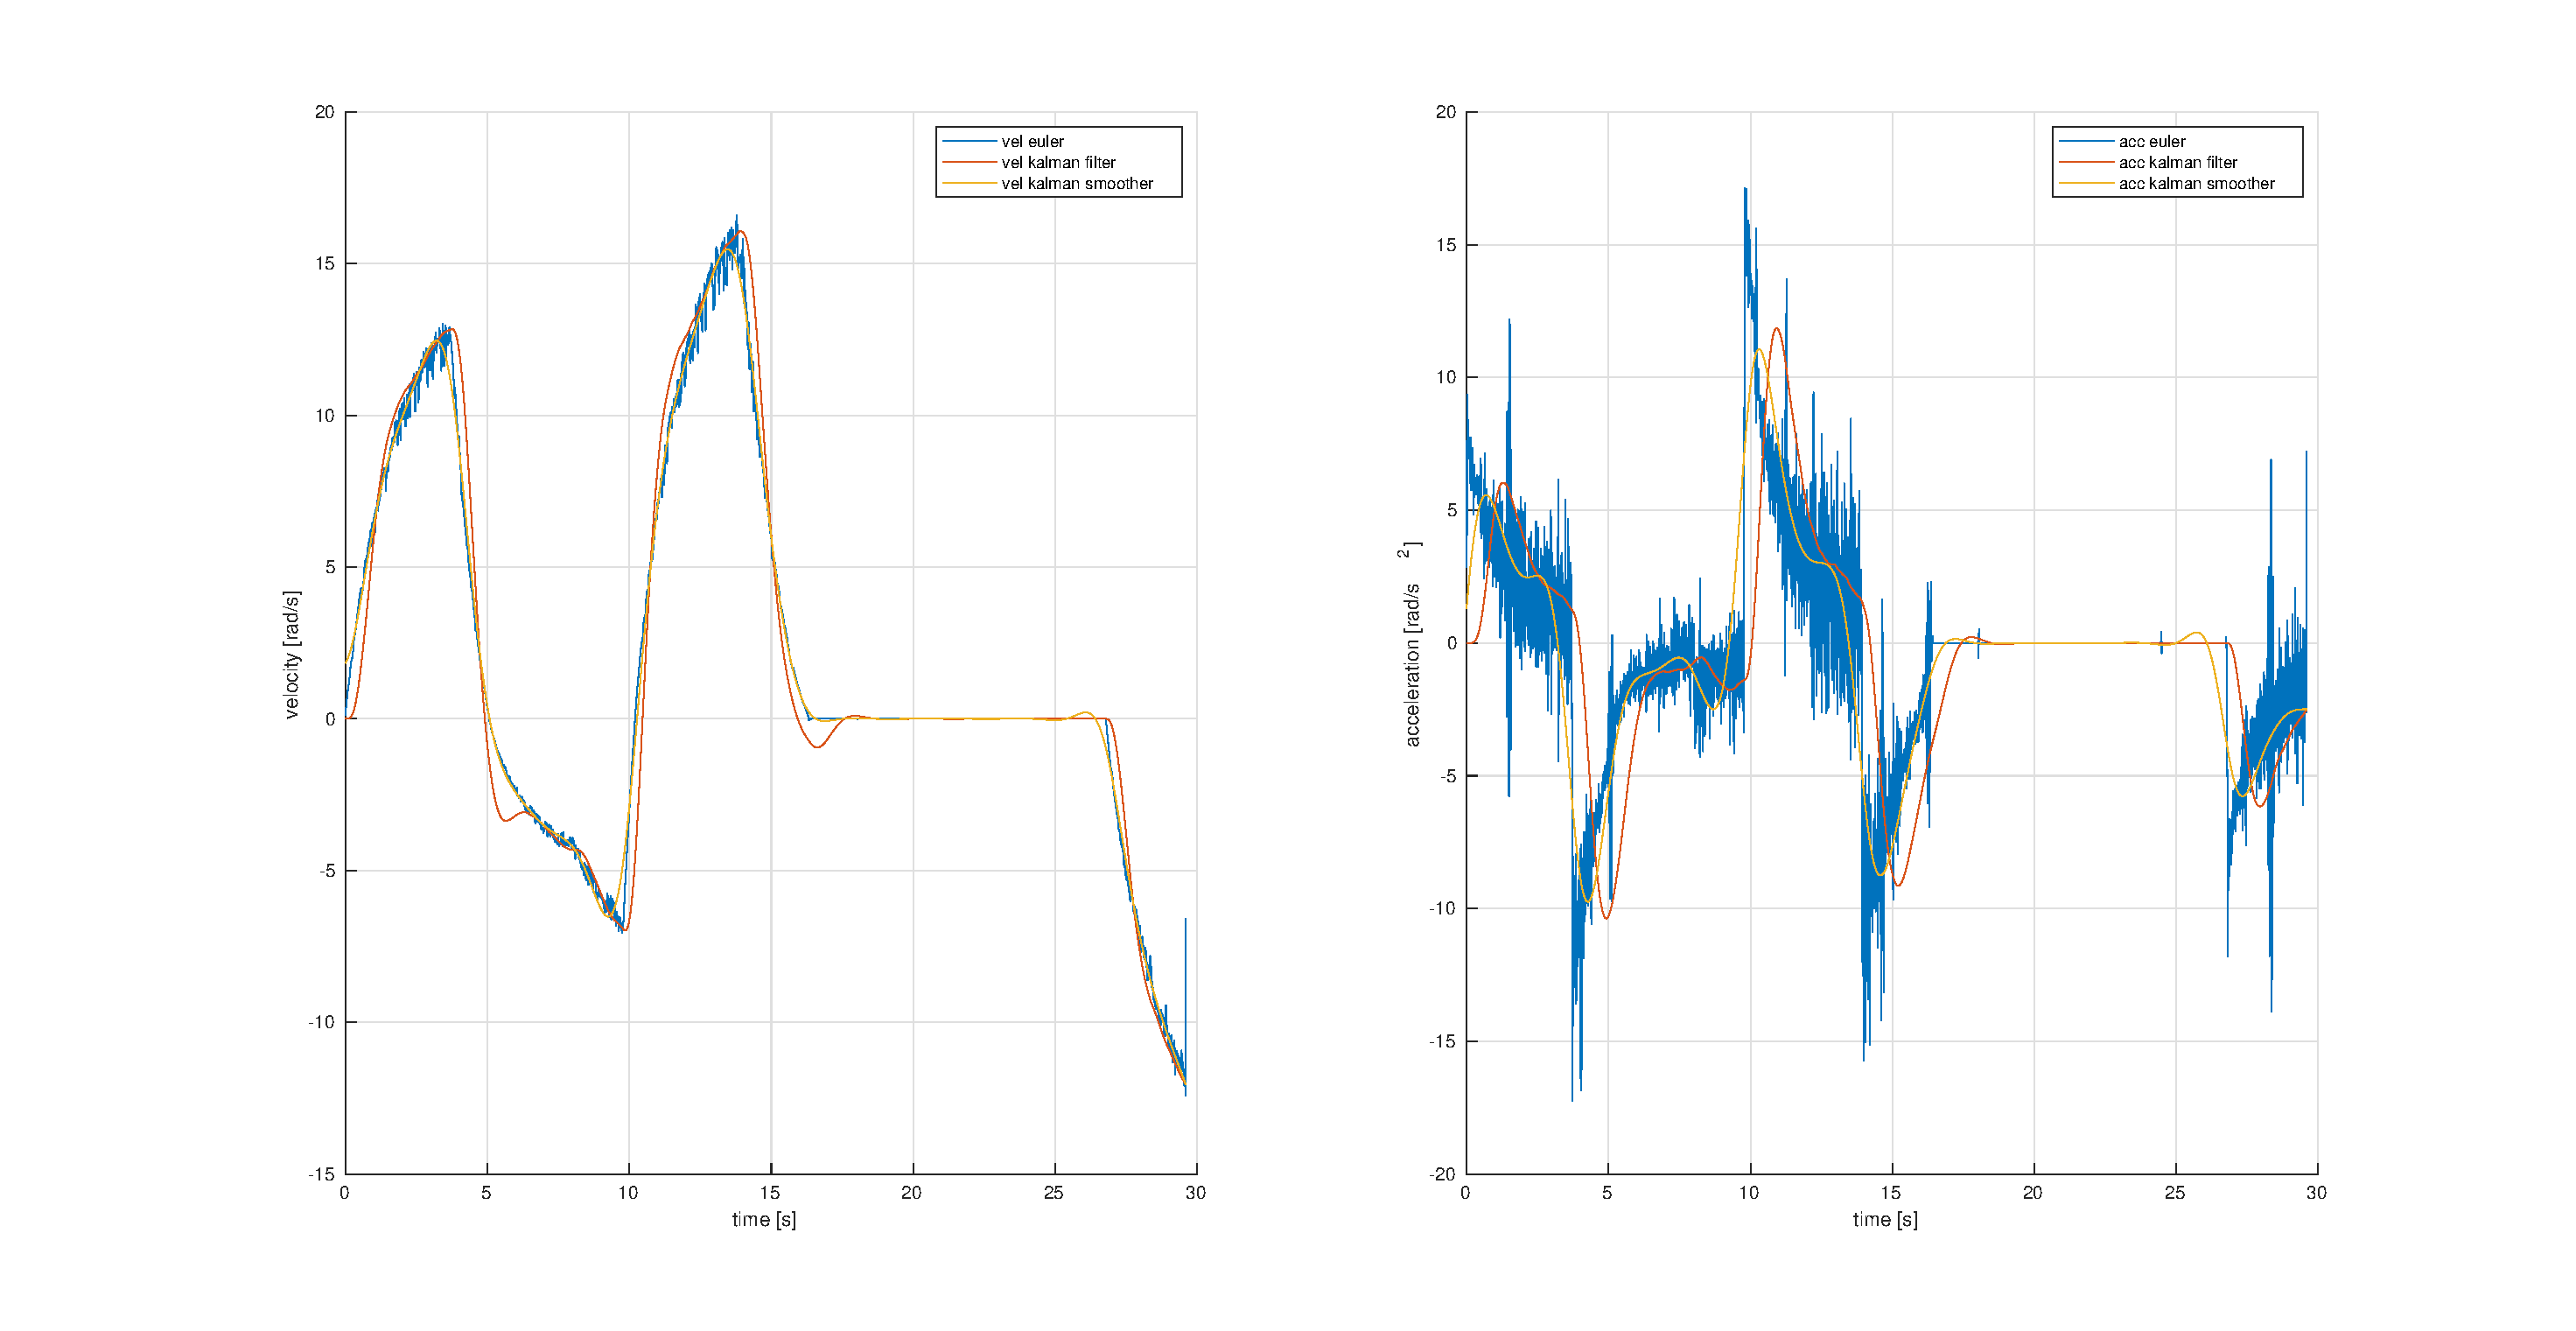
\includegraphics[scale=0.5]{images/kalman_smoother.eps}
    \end{center}
    \caption{Velocities and accelerations estimations using Kalman filter and Kalman Smoother}
    \label{fig:kalman_smoother}
\end{figure}
\section{HW 5: Least Square, RLS and Adaptive Estimation}
The aim of this section is to present three techniques to solve a gray-box indentification problem meaning that the class of the model is known but the specific parameters are unknown. If we consider a linear model:
\[
    y = x\beta \qquad \textit{for example a DC motor} \qquad V(t) = \begin{bmatrix}
        \dot{w}(t) & w(t) 
    \end{bmatrix} \begin{bmatrix}
        \tau/k \\ 1/k
    \end{bmatrix}
\]
the aim is to find the prediction:
\[
    \hat{y} = x \hat{\beta}
\]
where $\hat{\beta} \in \mathbb{R}^m$ is the matrix of coefficients that we have to determine.

\bigskip
\noindent The following methods are reported:
\begin{itemize}
    \item \textbf{Least square solution} $\hat{\beta} = (X^TX)^{-1}X^TY$ if $X^TX$ is nonsingular
    \item \textbf{Adaptive algorithm} $\hat{\beta}(k) = \hat{\beta}(k-1) + T_sgx^T(k)e(k)$ with $g > 0$. Basically we are moving in the opposite direction of the gradient of the minimized square error.
    \item \textbf{Recursive Least square} by solving the causal formulation:
\end{itemize}
\[
    \begin{cases}
        e(k) = y_k -x_k\hat{\beta}(k-1) \\
        P(k) = \frac{1}{\lambda} \left ( P(k-1) - \frac{P(k-1)x_k^Tx_kP(k-1)}{\lambda + x_kP(k-1)x_k^T}\right) \\ 
        K(k) = P(k)x_k^T \\
        \hat{\beta}(k) = \hat{\beta}(k-1) + K(k)e(k) 
    \end{cases}
\]
where $0 < \lambda \leq 1 $ is called forgetting factor

\begin{figure}[H]
    \begin{center}
        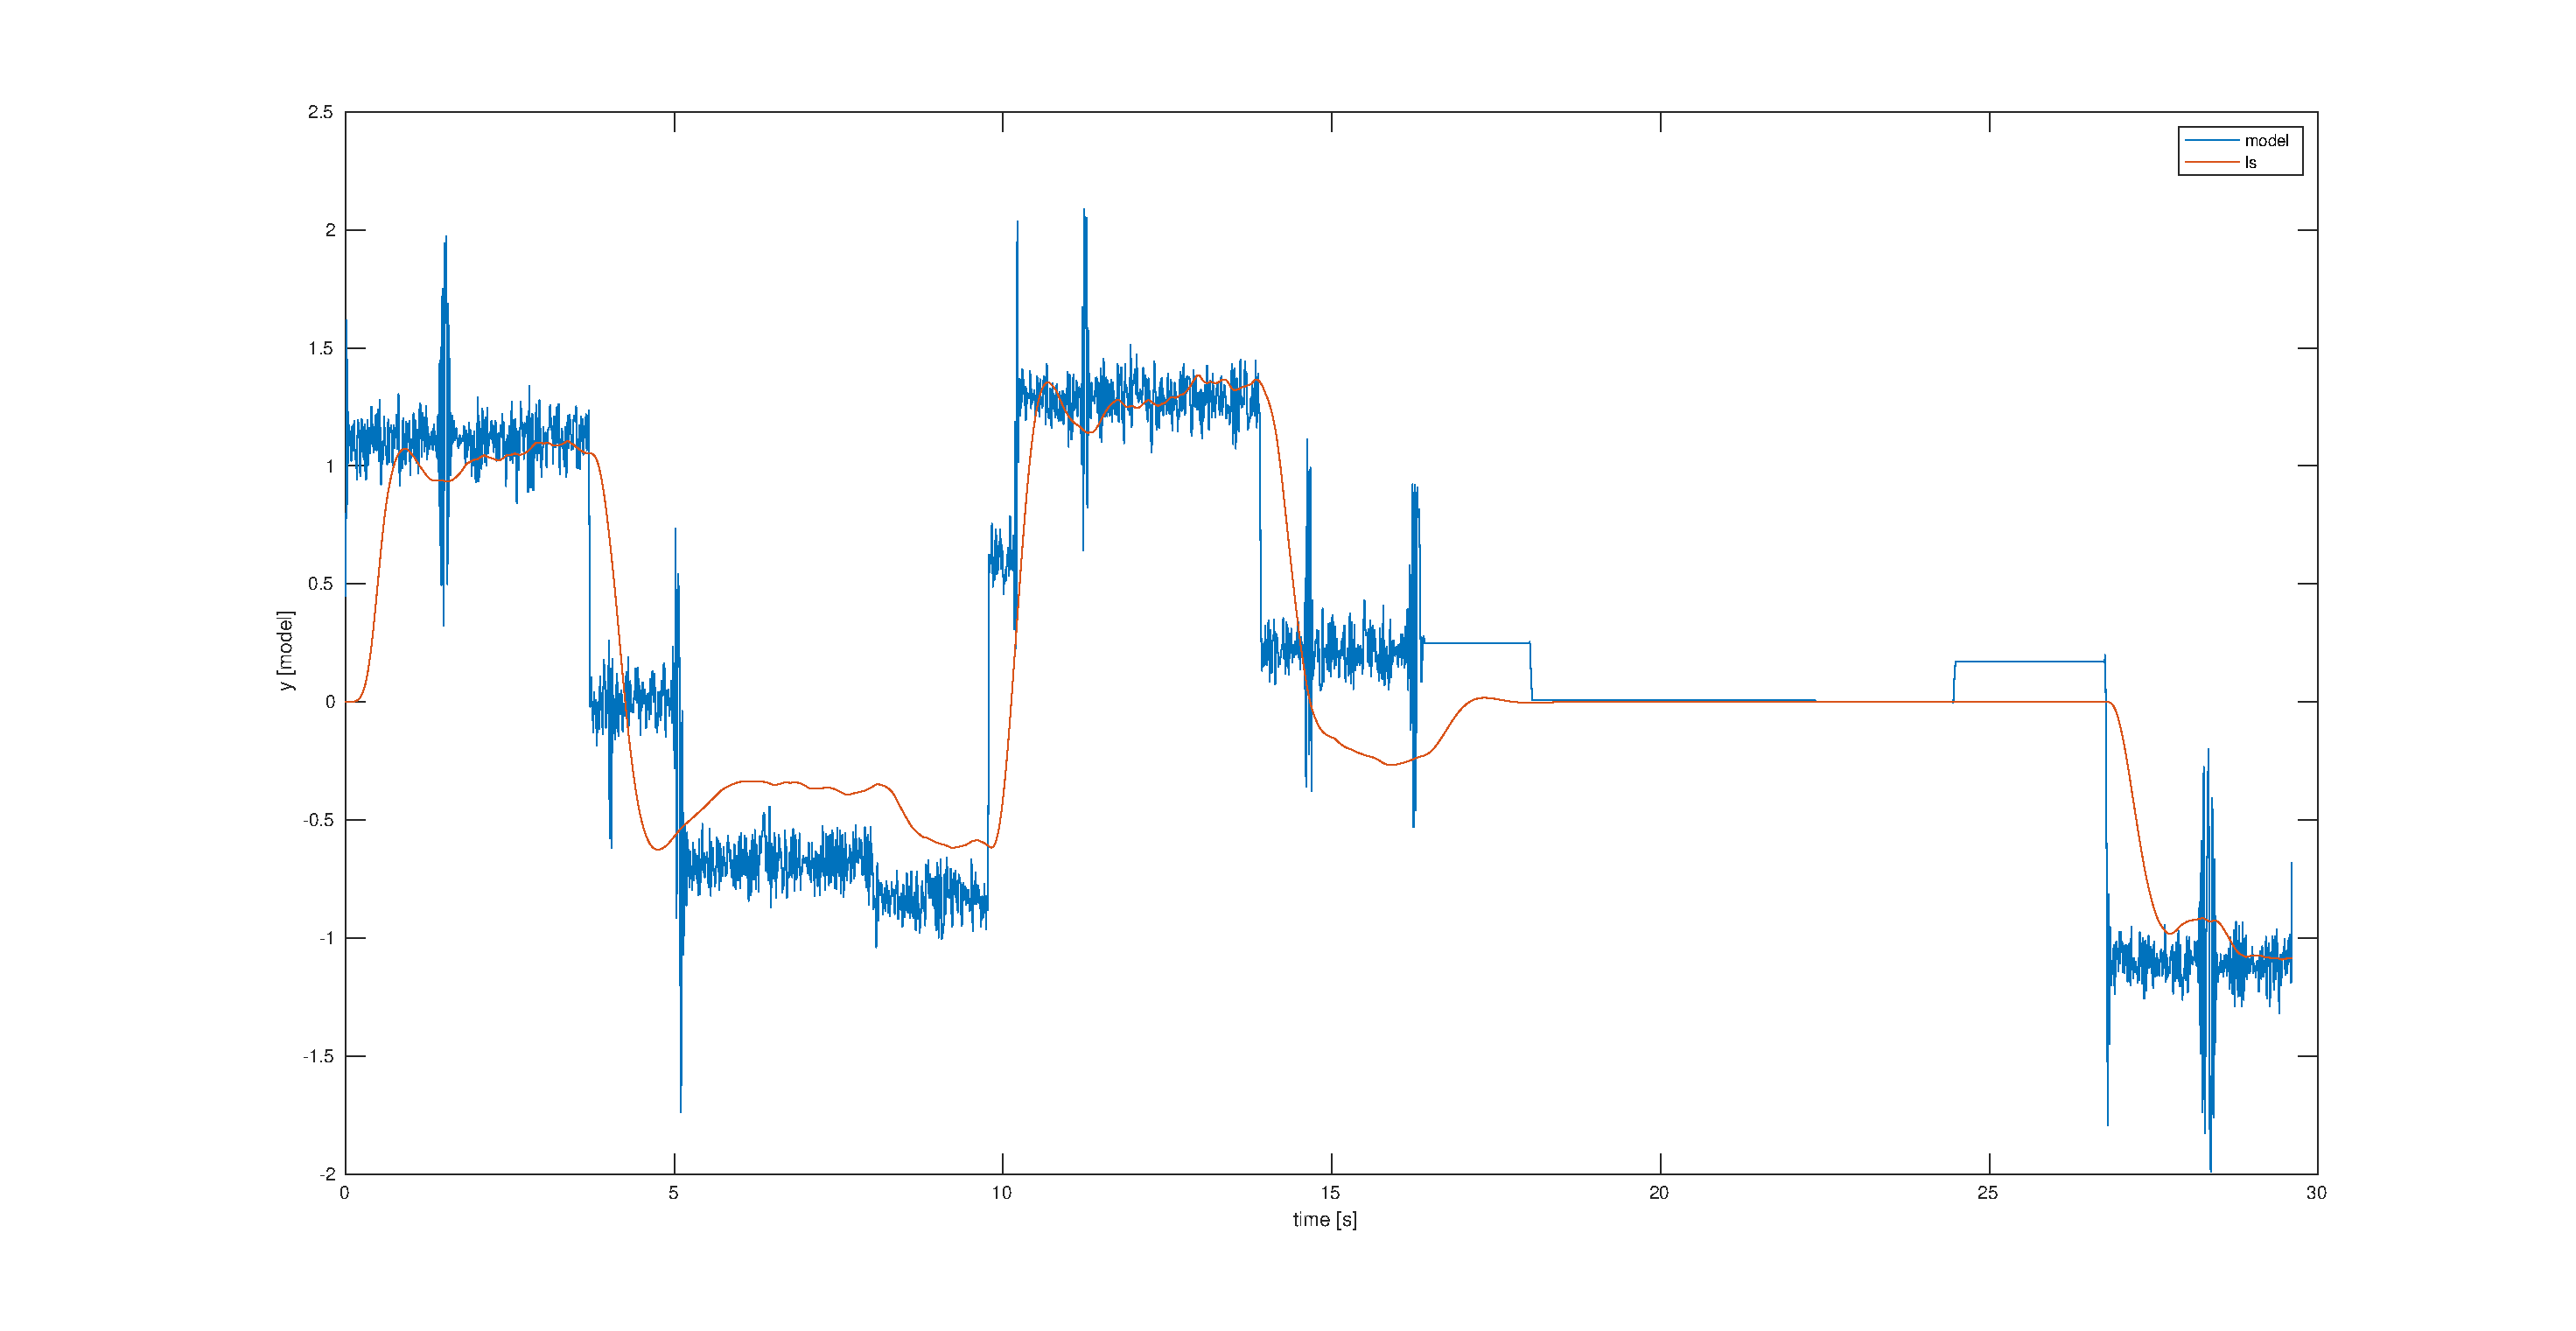
\includegraphics[scale=0.3]{images/ls.eps}
    \end{center}
    \caption{Least square estimation of the DC model of the motor}
    \label{fig:ls}
\end{figure}

\begin{figure}[H]
    \begin{center}
        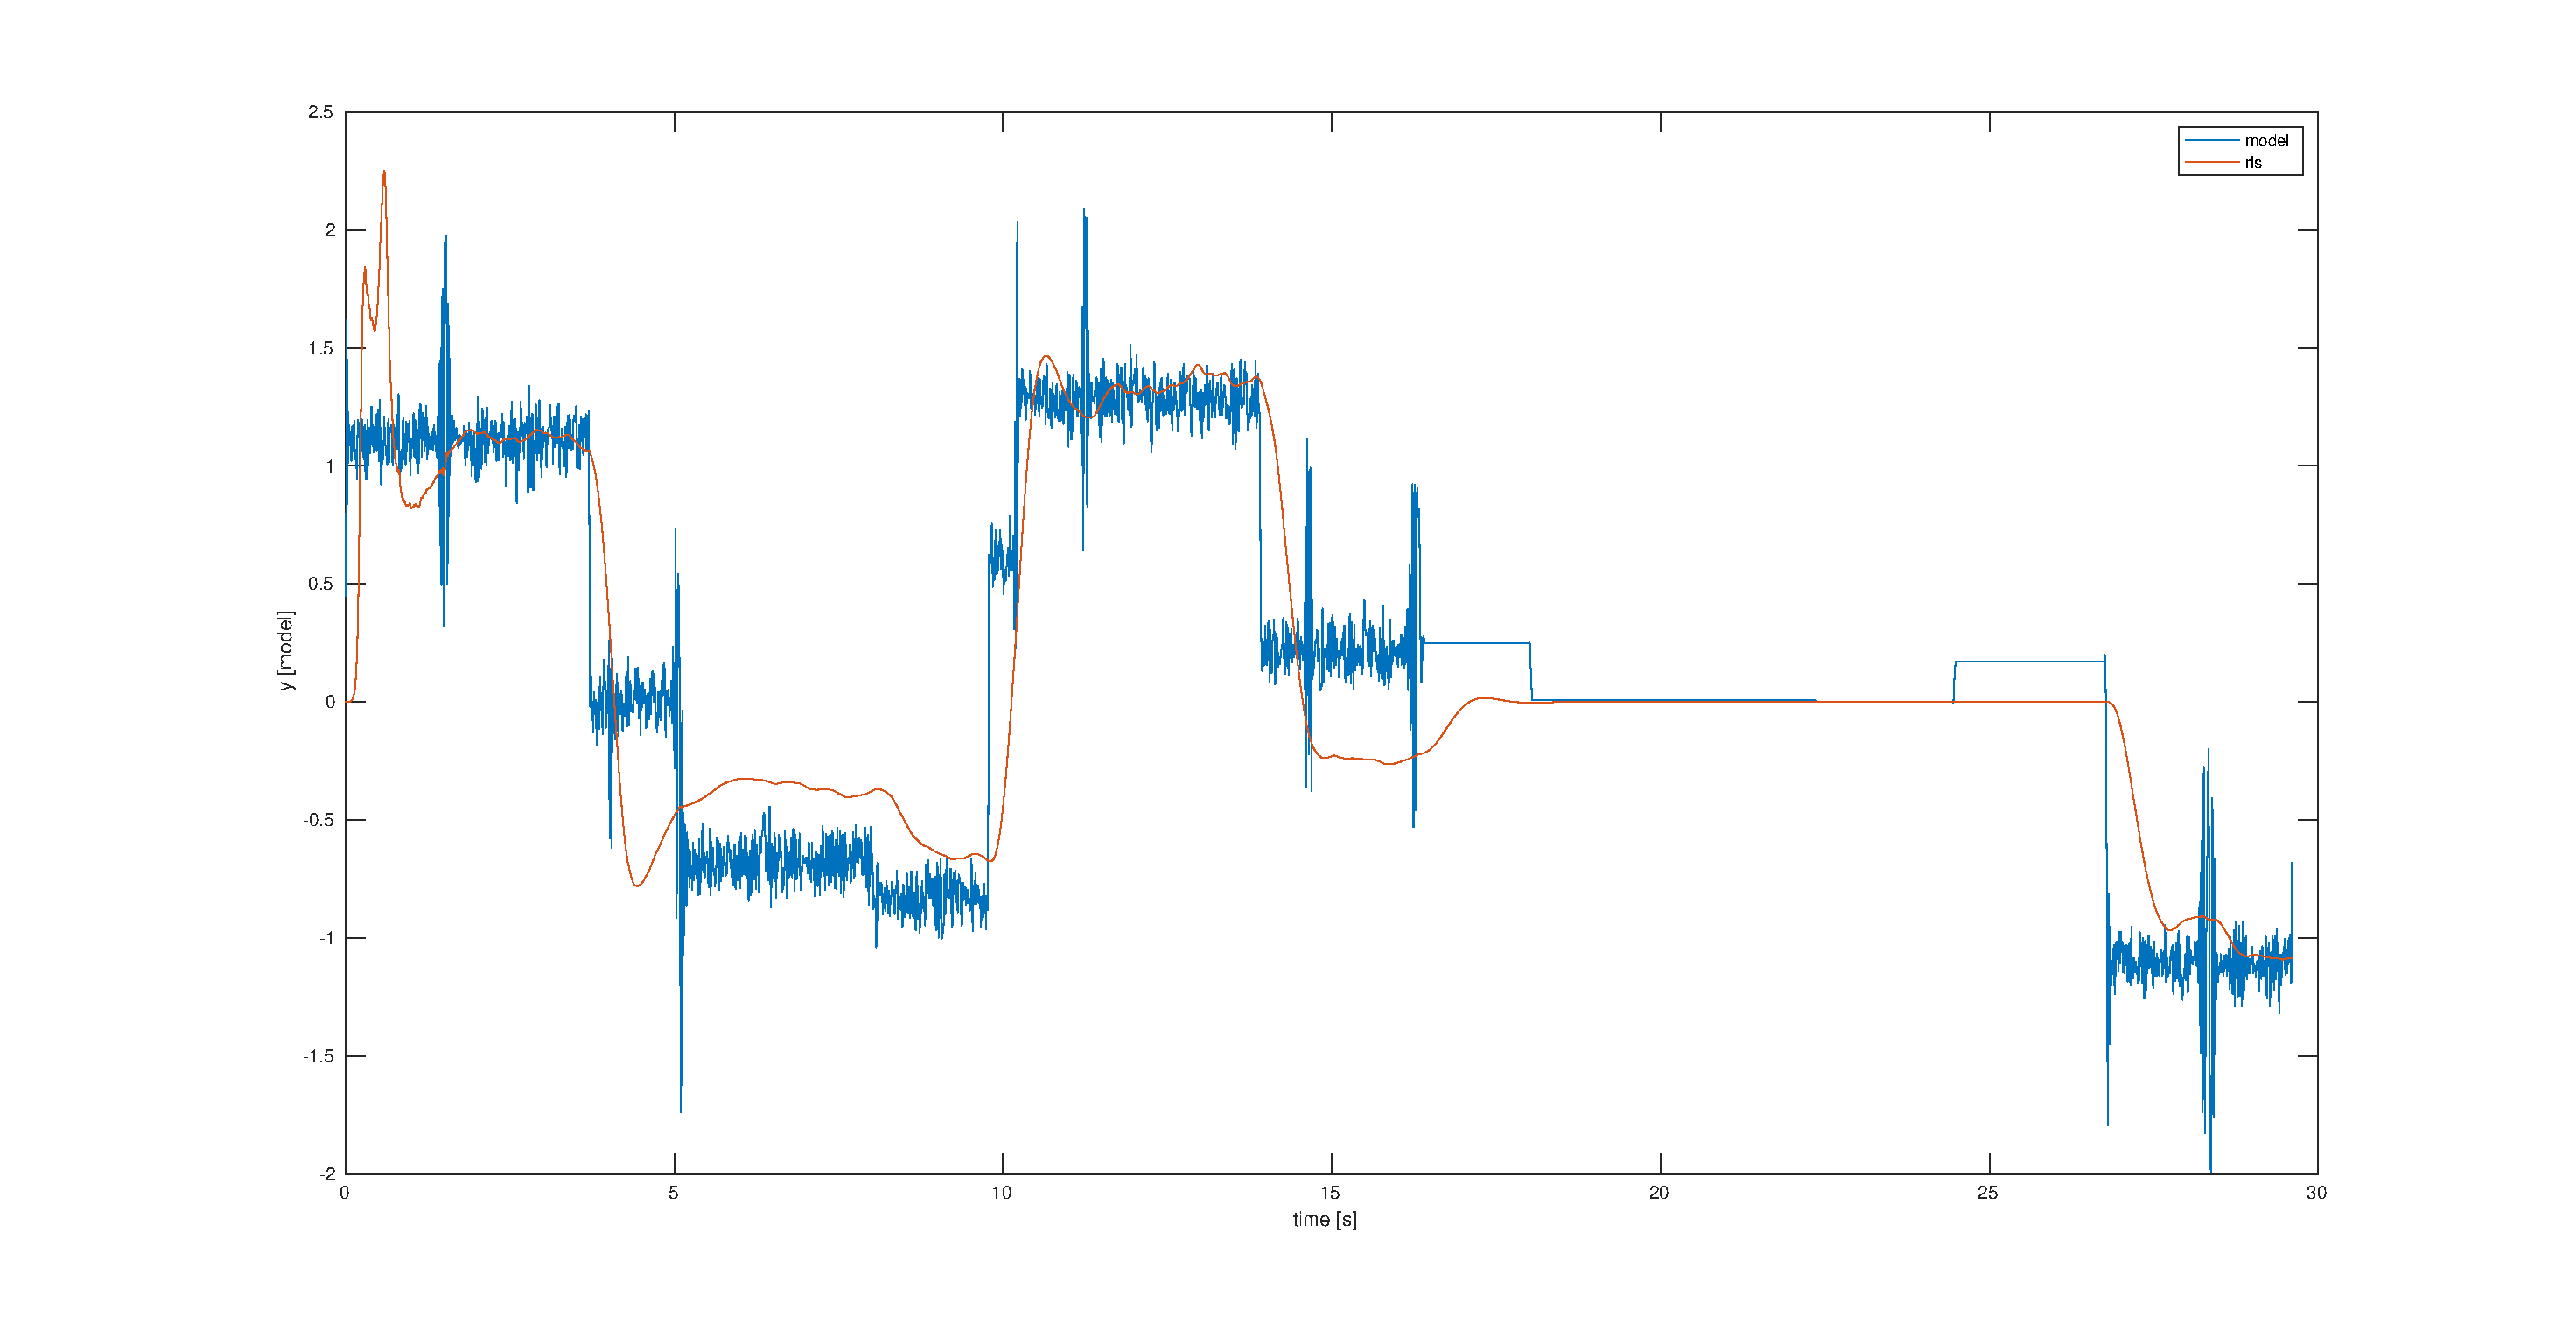
\includegraphics[scale=0.3]{images/rls.eps}
    \end{center}
    \caption{Recursive Least square estimation of the DC model of the motor}
    \label{fig:rls}
\end{figure}

\begin{figure}[H]
    \begin{center}
        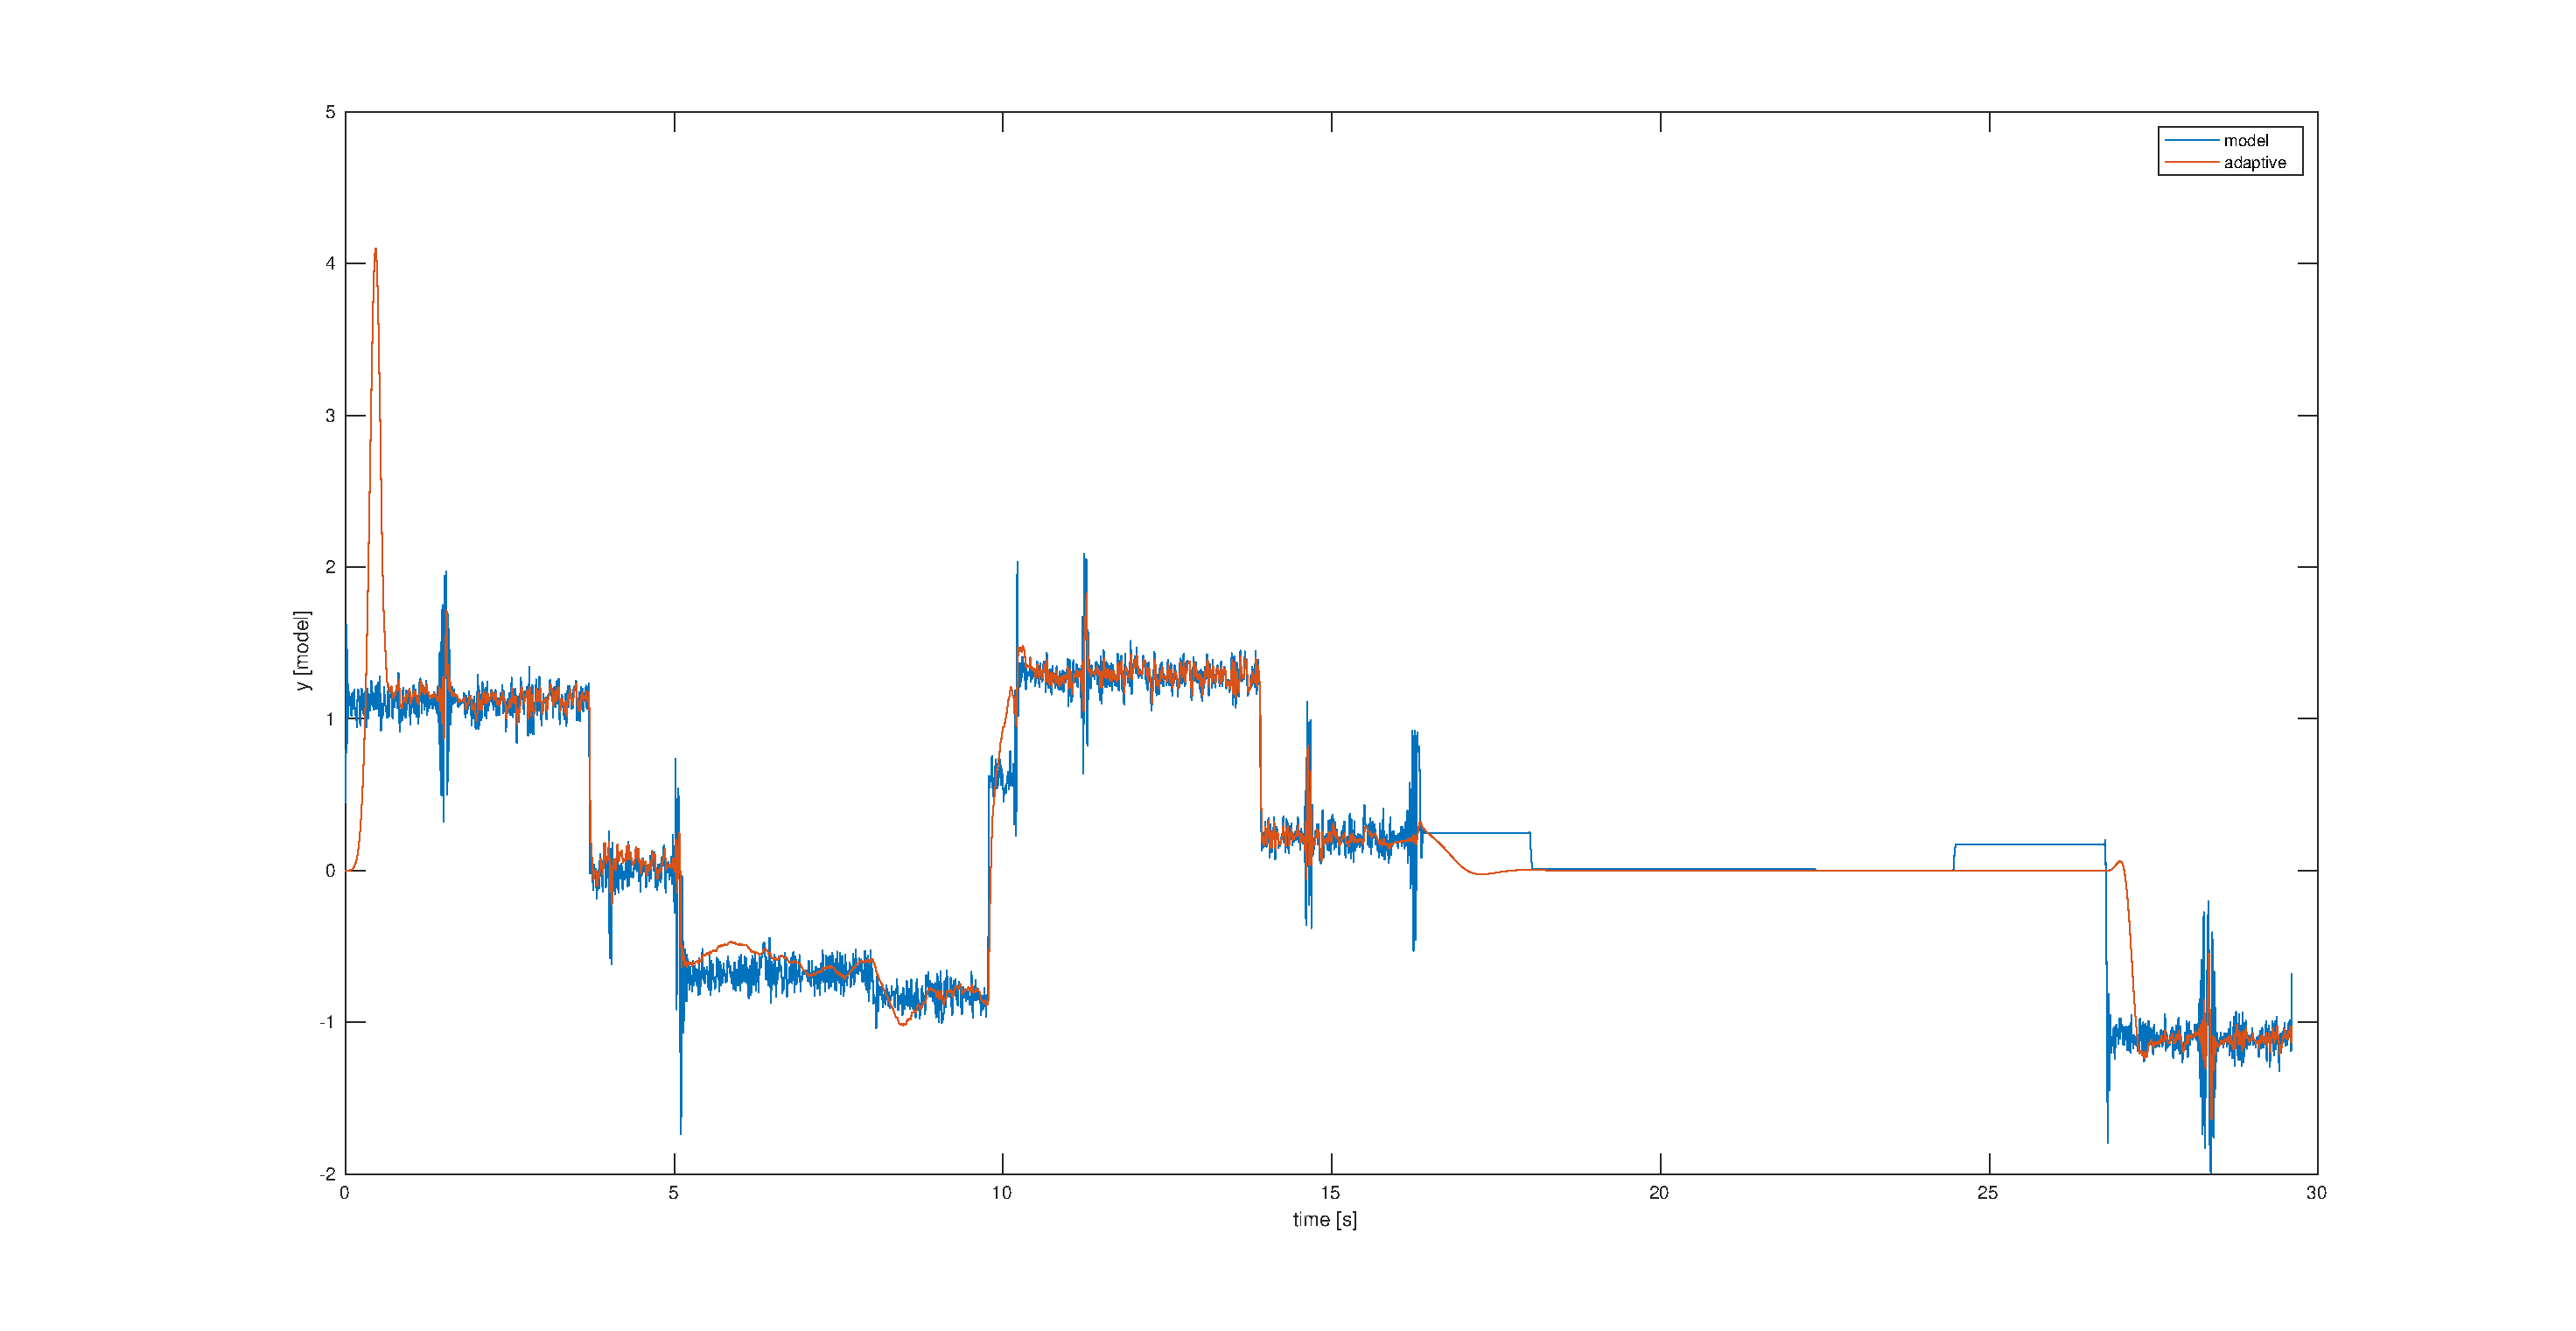
\includegraphics[scale=0.3]{images/adaptive.eps}
    \end{center}
    \caption{Adaptive estimation of the DC model of the motor}
    \label{fig:adaptive}
\end{figure}

\begin{figure}[H]
    \begin{center}
        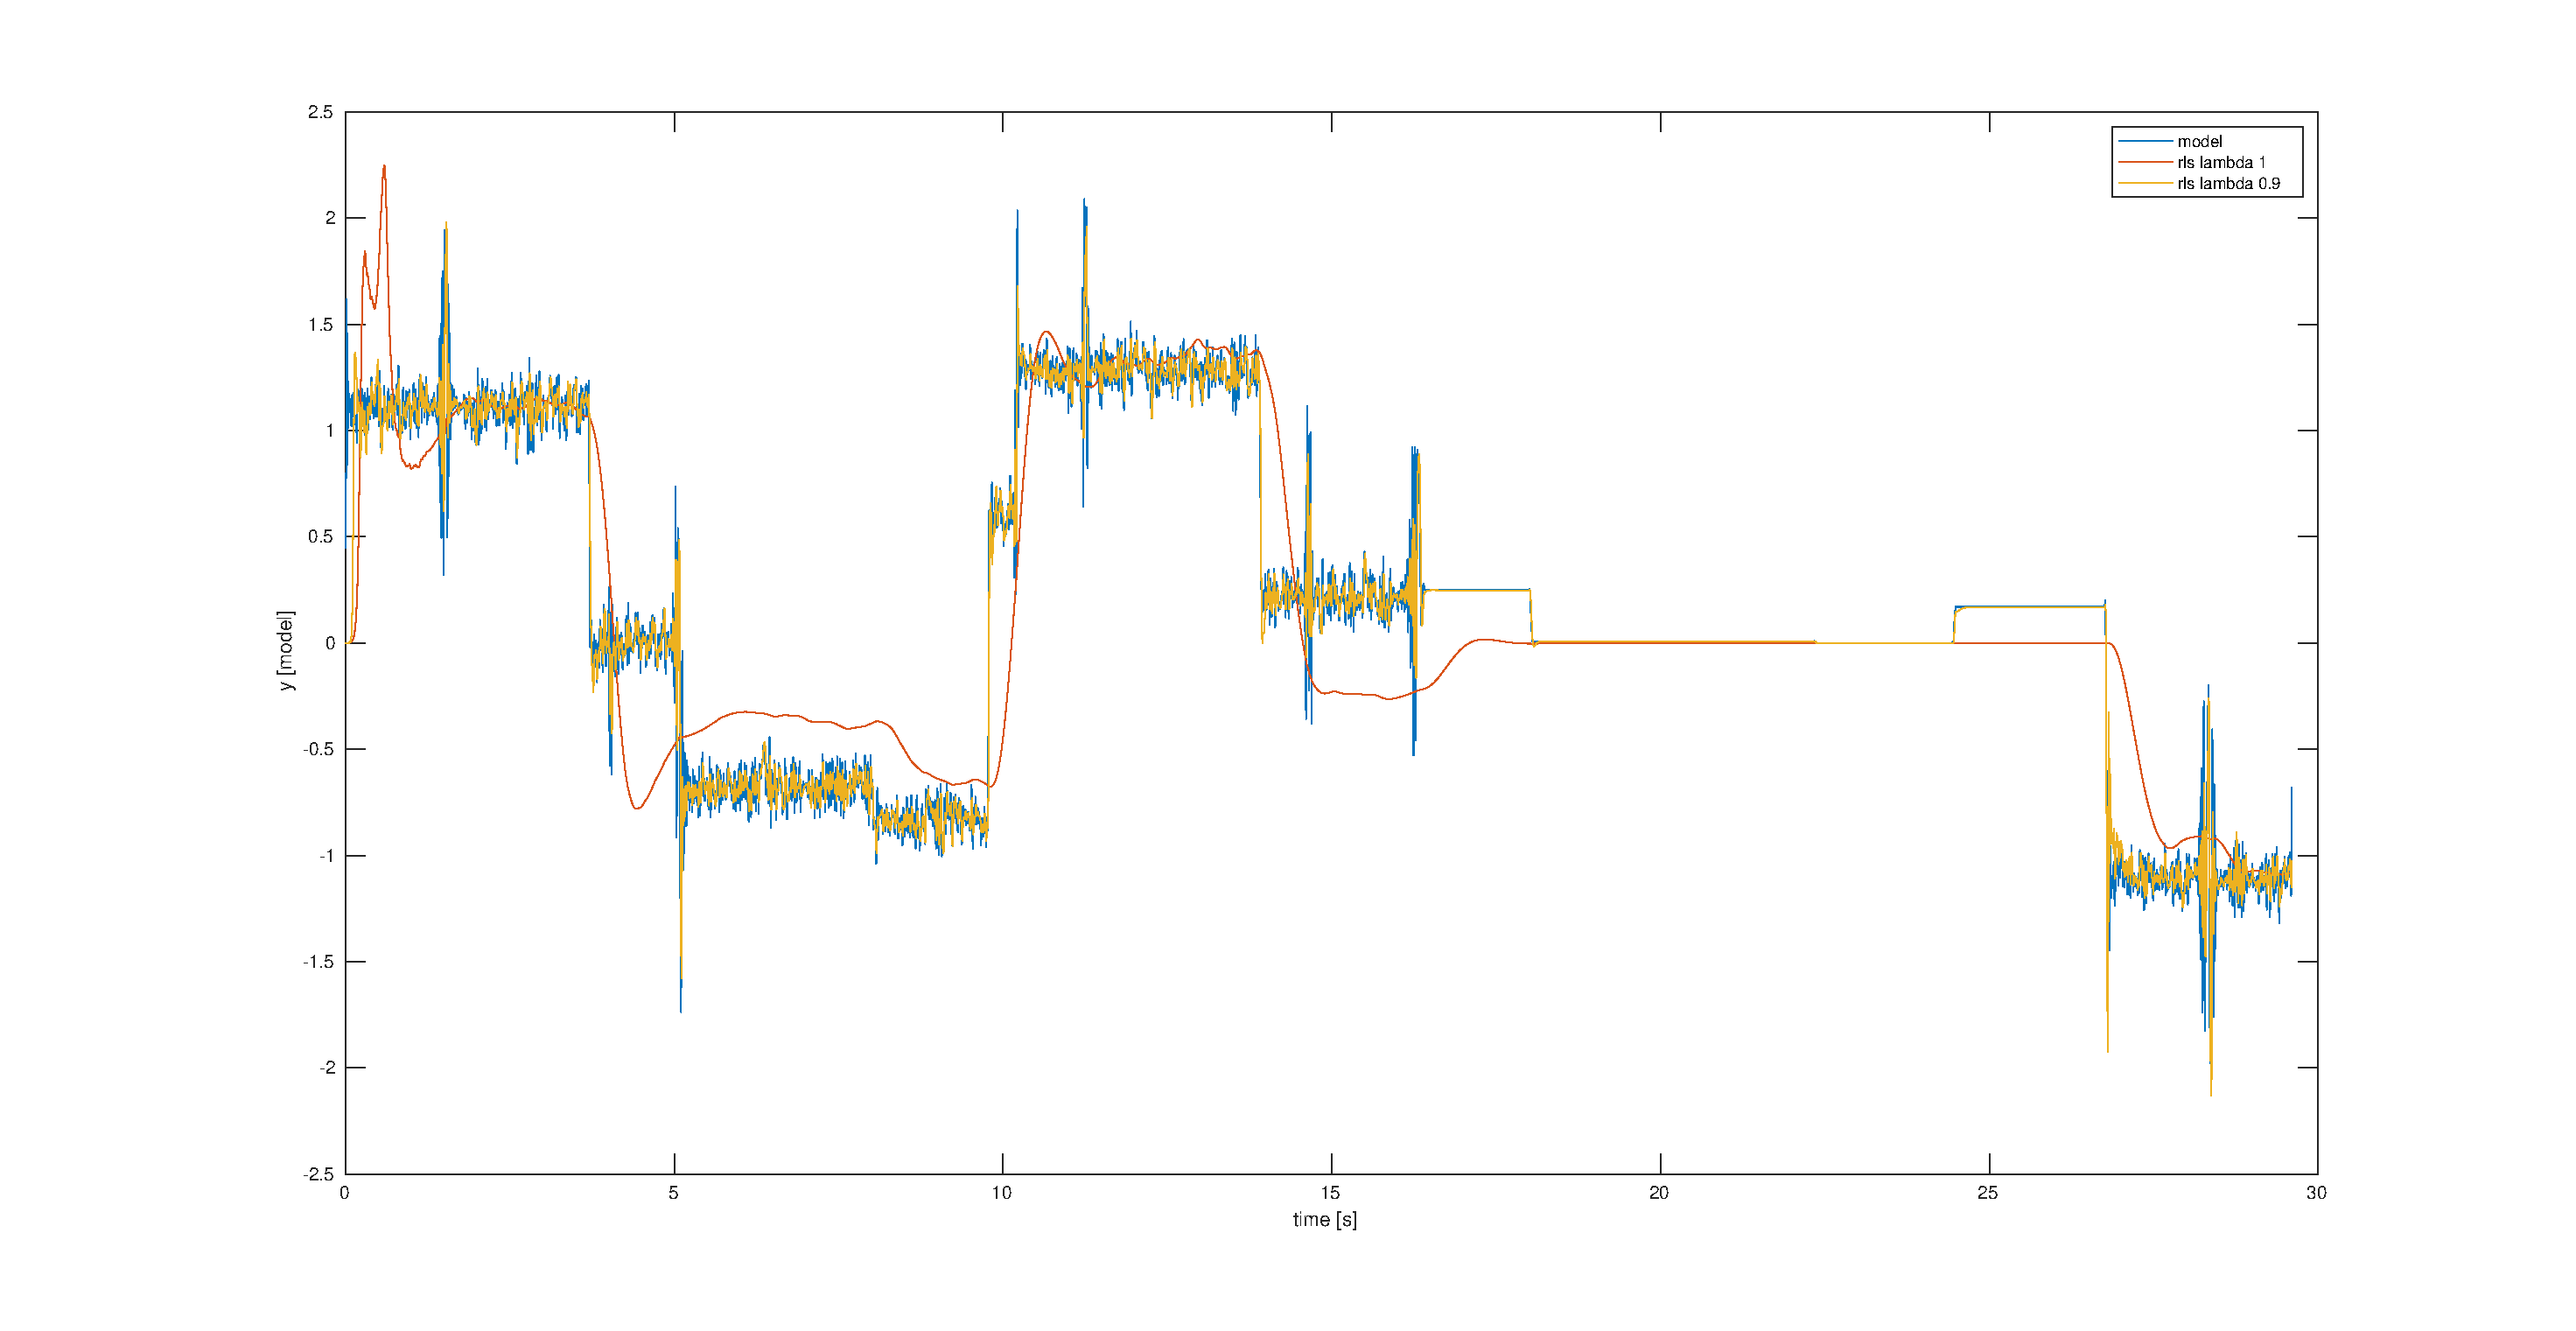
\includegraphics[scale=0.3]{images/rls_forget.eps}
    \end{center}
    \caption{Recursive Least square with forgetting factor of the DC model of the motor}
    \label{fig:rls_f}
\end{figure}

\section{Scattering based bilateral teleoperation architecture}
The core ideas in this architecture were described by Niemeyer and Slotine in Stable Adaptive Teleoperation (1991). The paper was \begin{quote}
    a preliminary study on how the existence of time-delays affects the application of advanced control shcemes to effective force-reflecting telerobotic systems.
\end{quote}

The fondamental ideas are developed in the context of passivity formalism which
\begin{quote}
    represents a mathematical description of the intuitive physical concepts of power and energy. It provides a simple and robust tool to analyze the stability of a nonlinear system while maintaining global stability properties.
\end{quote}
A system is said passive if:
\[
    P = x^Ty = \frac{dE}{dt} + P_{diss}
\]
and it is also true that:
\[
    \int_{0}^{t} P \,d\tau = \int_{0}^{t} x^Ty \,d\tau = E(t) - E(0) + \int_{0}^{t} P_{diss} \,d\tau \geq -E(0) = \text{constant}
\]

The interesting properties of passivity formulations are its closure properties via feedback or parallel configuration. Moreover 

\begin{quote}
    the use of passivity is a sufficient condition for the stability of the system coupled to a passive environment with a bounded operator input energy.
\end{quote}

The wave variable formulation, formally treated in scattering theory, is introduced. In this context a system is passive if the energy provided by the output waves is limited to the energy received via input waves
\[
    \int_{0}^{t} \frac{1}{2}v^Tv \,d\tau \leq \int_{0}^{t} \frac{1}{2}u^Tu \,d\tau 
\]
The transformations used to map $(\dot{x},F)$ into $(u,v)$ are:
\[
    u_l = \frac{1}{\sqrt{2b}}(F_l + b \dot{x_l}) \qquad u_r = \frac{1}{\sqrt{2b}}(F_r - b \dot{x_r}) 
\]

\[
    v_l = \frac{1}{\sqrt{2b}}(F_l - b \dot{x_l}) \qquad v_r = \frac{1}{\sqrt{2b}}(F_r + b \dot{x_r}) 
\]
they can be used to extract the desired configurations based on the signal provided such as forces or velocities.
\subsection{Scattering based PF}
\end{document}
